%----------------------------------------------------------------------------------------
%	Metropolia Thesis LaTeX Template
%----------------------------------------------------------------------------------------
% License:
% This work is licensed under the Creative Commons Attribution 4.0 International License.
% To view a copy of this license, visit http://creativecommons.org/licenses/by/4.0/.
%
% However, this license apply to this template. As a template, it is supposed to be
% modified for your own needs (with your thesis content). For this reason, if you use
% this project as a template and not specifically distribute it as part of a another
% package/program, we grant the extra permission to freely copy and modify these files as
% you see fit and even to delete this copyright notice.
% In short, you are free to publish your thesis under whatever license you wish, even
% keep the all rights reserved to you.
%
% Authors:
% Panu Leppäniemi, Patrik Luoto, Mikaa Oni and Patrick Ausderau
%
% Credits:
% Panu Leppäniemi: abstract, def, cleaning,...
% Patrik Luoto: title page, abstract in Finnish, abbreviation, math,...
% Mikaa Oni: switch to biber biblatex
	% Patrick Ausderau: initial version, style, table of content, bibliography, figure,
%                   appendix, table, source code listing,...
%
% Please:
% If you find mistakes, improve this template and alike, please contribute by sharing
% your improvements and/or send us your feedback there:
% https://github.com/panunu/metropolia-thesis-latex
% And of course, if you improve it, add yourself as an author.
%
% Compiler:
% Use XeLaTeX as a compiler. LuaLaTeX works too.
% Typical compilation:
% # minted require -shell-escape to run  external script.
% # -8bit avoid ^^I for tabs in minted.
% $ xelatex -shell-escape -8bit main
% # If any change in the bibliography
% $ biber main
% # If any change with the abbreviation or acronym
% $ makeglossaries main
% #Then compile again
% $ xelatex -shell-escape -8bit main
% #And if still some citation or label warnings, compile once more
% $ xelatex -shell-escape -8bit main

%----------------------------------------------------------------------------------------
%	THESIS INFO
%----------------------------------------------------------------------------------------

% All general information (main language, title, author (you), degree programme, major
% option, etc.)
% Edit the file chapters/0info.tex to change these information
\documentclass[12pt,a4paper,oneside,article]{memoir}%Do not touch this first line ;)
% add hidelinks to documentclass to remove link boxes
% Global information (title of your thesis, your name, degree programme, major, etc.)

\def\bilingual{no}%For Finnish students, you must have 2 abstracts, one in English and one in your native language (Finnish or Swedish), so "yes", your thesis is bilingual.
%\def\bilingual{no}%For international student writing in English, only one language and one abstract.

%\def\thesislang{finnish} %change this depending on the main language of the thesis.
\def\thesislang{english} % "english" is the only other supported language currently. If someone has the swedish, please contribute!

\def\secondlang{english} %if the main language is Finnish (or Swedish), you must have 2 abstracts (one in Finnish (or Swedish) and one in English)
%\def\secondlang{finnish}
%If the main language is English and that you are native Finnish (or Swedish) speaker, you must have also abstract in your native language on top of the English one.

\author{Visa Harvey} %your first name and last name

%\def\alaotsikko{Alaotsikko/Subtitle} %DISABLED, seems not to be an option with the 2018 template. If you really need it, uncomment and modify style/title.tex accordingly.

%License
%When publishing your thesis to theseus.fi, you can keep all rights reserved to you,
%or use one of the Creative Commons https://creativecommons.org/licenses/?lang=en
%This attribute will set the license in the metadata of the generated pdf.
%possible options (case sensitive):
%all (keep all rights reserved to yourself)
%by (Attribution)
%by-sa (Attribution-ShareAlike)
%by-nd (Attribution-NoDerivs)
%by-nc (Attribution-NonCommercial)
%by-nc-sa (Attribution-NonCommercial-ShareAlike)
%by-nc-nd (Attribution-NonCommercial-NoDerivs)
%Note that theseus do not accept dedication to public domain CC0
\def\thesiscopy{all}

%Finnish section, for title/abstract
\def\otsikko{Opinnäytetyön otsikko}
\def\tutkinto{Tutkinto (esim. Insinööri (AMK))} % change to your needs, e.g. "YAMK", etc.
\def\kohjelma{Koulutusohjelma (esim. Tieto\textendash ja viestintätekniikka)}
\def\suuntautumis{Ammatillinen pääaine (esim. Mobile Solutions)}
\def\thesisfi{Insinöörityö}%was Opinnäytetyö
\def\ohjaajat{
Titteli Etunimi Sukunimi\newline
Titteli Etunimi Sukunimi
}
\def\tiivistelma{
Tämä on tiivistelmän ensimmäinen kappale. Tiivistelmän kappaleet loppuvat komentoon newline, jotta saadaan yksi tyhjä rivi aikaiseksi. \newline

Tämä on tiivistlemän toinen kappale.
}
\def\avainsanat{avainsana, avainsana}
\def\aihe{Lyhyt kuvaus opinnäytetyöstä. Max 255 merkkiä.}%for the pdf metadata/properties. If not used, empty it and also the \def\subject.

%English section, for title/abstract
\title{Automated device for Raspberry Pi Pico recovery}
\def\metropoliadegree{Bachelor of Engineering} % change to your needs, e.g. "master", etc.
\def\metropoliadegreeprogramme{Information Technology}
\def\metropoliaspecialisation{Smart Systems}
\def\thesisen{Bachelor’s Thesis} % change to your need, e.g. master's
\def\metropoliainstructors{
Keijo Länsikunnas, Principal Lecturer\newline
Anne Pajala, Assistant advisor
}
\def\abstract{
The aim of this project is to create Raspberry Pi Pico recovery platform, able to initialise and recover a target Pi Pico development board to initial usable state or recover a MicroPython installation from a non accessible or booting startup script.
\newline

The software functionality side of this thesis was achieved, with further hardware development still needed to achieve a practical usable solution.
\newline

}
\def\metropoliakeywords{SWD, Raspberry Pi Pico, USB Virtual File System}
\def\subject{short description of the thesis. Max 255 characters.}%for the pdf metadata/properties. If not used, empty it and also the \def\aihe.


%----------------------------------------------------------------------------------------
%	GLOBAL STYLES
%----------------------------------------------------------------------------------------

% If you need extra package, etc. modify the style/style.tex file.
% If you are using Windows OS, you will need to change default font to Arial in that
% style/style.tex file (or install Liberation Sans font to your system).
% If you are using MacOS or linux, make sure you have Liberation Sans font installed.
% Global style. Normally should not be edited.
% If you use windows OS, eventually change \setmainfont to Arial
% Check around commit https://github.com/panunu/metropolia-thesis-latex/commit/a0c15ac77bab1a52c59c517a18080938e57bf5ef
% to see how the font files were manually added (after downloading them: https://pagure.io/liberation-fonts/ )

%\usepackage[l2tabu, orthodox]{nag}%check for obsolete packages (with outdated nag package?)

%condition e.g. for adding or not space in TOC,...
\usepackage{etoolbox}
\ifdefstring{\bilingual}{yes}{
  \usepackage[\secondlang,\thesislang]{babel}% finnish (or swedish) and english
}{
  \usepackage[\thesislang]{babel}% english only
}
\usepackage{iflang}
\usepackage{amsmath}
\usepackage{amsfonts}%extra mathematical symbols
\usepackage{amssymb}
\usepackage{fontspec}
\usepackage{titlesec}
\usepackage{mathtools}%enhance the appearance of documents containing a lot of mathematics
\usepackage[amssymb]{SIunits}
\usepackage[version=3]{mhchem}
\usepackage{tikz} % mindmaps, flowcharts, piecharts, examples at http://www.texample.net/tikz/examples/
\usetikzlibrary{shapes.geometric, arrows}

\usepackage{ragged2e}
\IfLanguageName{finnish}{
  \RaggedRight%2021 template, align left and hyphennization for Finnish version
  \setlength{\RaggedRightRightskip}{0pt plus 1fil}%TODO: fix the Overfull/Underfull warnings when \RaggedRight (likely in title and abstact)
}{}
\makeatletter
  \let\@gnewline\@raggedtwoe@saved@gnewline% Restore original functionality of \newline
  \let\\\@raggedtwoe@savedcr% Restore original functionality of \\
\makeatother

%for compact list
\usepackage{enumitem}
%\usepackage{verbatim}%for block comment
%forcing single line spacing in bibliography
\DisemulatePackage{setspace}
\usepackage{setspace}
%\usepackage{eurosym}%euro symbol
%try to count
\usepackage{totcount}
%insert source code
%require -8bit -shell-escape in the xelatex compile command
%if compiling locally, consider options cachedir=minted,outputdir=~/.tex
\usepackage[newfloat]{minted}
\setminted{tabsize=2,linenos,breaklines,breaksymbolleft={\quad},baselinestretch=1}
\setmintedinline{breaklines,breakanywhere}
\usepackage[singlelinecheck=false]{caption}
%force the width of a table instead of column
\usepackage{tabularx}
\usepackage{booktabs} %why not booktabs? :3

\usepackage{csquotes}% avoid warning with babel

\usepackage{float} % For forced figure location with modifier H (\begin{figure}[H])
\usepackage{wrapfig}

% citep-macro for reference with period inside square brackets [1.]
\newcommand{\citep}[1]{
 \renewcommand\citeright{.]}
 \cite{#1}
 \renewcommand\citeright{]}
}

%set date format to D.M.YYYY
\def\pvm{\the\day.\the\month.\the\year}
%set date format to D Month YYYY
\usepackage[en,useregional=false]{datetime2}
\DTMsetup{datesep=.}
\DTMnewdatestyle{dMonthyyyy}
{%
  \renewcommand{\DTMdisplaydate}[4]{%
    \number##3 % day
    ~% separator
    \DTMenglishmonthname{##2}% month name
    ~% separator
    \number##1% year
  }%
  \renewcommand{\DTMDisplaydate}[4]{%
    \DTMdisplaydate{##4}{##3}{##2}{##1}%
  }%
}
\DTMsetdatestyle{dMonthyyyy}
\date{\today}

\newcommand\tn[1]{\textnormal{#1}} %use \tn instead of \textnormal
\newcommand\reaction[1]{\begin{equation}\ce{#1}\end{equation}} %\reaction{} for chemical reactions

%NORMAL TEXT
%all text, title, etc. in the same font: Arial
%NOTE: fontname is case-sensitive
\setmainfont[Scale=0.98]{Liberation Sans}
%line space
\linespread{1.46}
\AtBeginEnvironment{tabular}{\singlespacing}
%\doublespacing
%margin
%geometry moved after hyperref
\setlength{\parindent}{0pt} %first line of paragraph not indented
\setlength{\parskip}{16.5pt} %one empty line to separate paragraph
%list with small line space separation
\tightlists
\setlist[itemize]{before=\singlespacing,itemsep=6pt,leftmargin=63pt,labelsep=22pt,topsep=1.5pt,partopsep=0pt,after=\vspace{-22pt}\newline}
\setlist[enumerate]{before=\singlespacing,itemsep=6pt,leftmargin=63pt,labelsep=22pt,topsep=1.5pt,partopsep=0pt,after=\vspace{-22pt}\newline}

%IMAGE - FIGURE
%the figures should be placed in the "illustration" folder
\graphicspath{{illustration/}}
%figure number without chapter (1.1, 1.2, 2.1) to (1, 2, 3)
\counterwithout{figure}{chapter}
%border around images
\setlength\fboxsep{0pt}
\setlength\fboxrule{0.5pt}
%space after figure caption (and other float elements)
\setlength{\belowcaptionskip}{-7pt}
\setlength{\intextsep}{16.5pt}%space around floats
\AtBeginEnvironment{table}{\addvspace{16.5pt}}

%TABLE
\counterwithout{table}{chapter}

%SOURCE CODE
\newenvironment{code}{\captionsetup{type=listing}}{}
\IfLanguageName{finnish}{\SetupFloatingEnvironment{listing}{name=Koodiesimerkki}}{}%was Listaus
%\counterwithout{lstlisting}{chapter}
%moved after begin document, otherwise does not compile

%TOC
%change toc title
\IfLanguageName{finnish}{\addto{\captionsfinnish}{\renewcommand*{\contentsname}{Sisällys}}}{}
%remove dots
\renewcommand*{\cftdotsep}{\cftnodots}
%chapter title and page number not in bold
\renewcommand{\cftchapterfont}{\normalfont}
\renewcommand{\cftchapterpagefont}{\normalfont}
%sub section in toc
\setcounter{tocdepth}{2}
%subsection numbered
\setcounter{secnumdepth}{2}
\renewcommand{\tocheadstart}{\vspace*{-33.5pt}}
\renewcommand{\printtoctitle}[1]{\fontsize{13.5pt}{13.5pt}\bfseries #1\vspace*{-4pt}}
%\renewcommand{\aftertoctitle}{\vspace*{-22pt}\afterchaptertitle}
%spacing after a chapter in toc
\preto\section{%
  \ifnum\value{section}=0\addtocontents{toc}{\vskip11pt}\fi
}
%spacing after a section in toc
\renewcommand{\cftsectionaftersnumb}{\vspace*{-3pt}}
%spacing after a subsection in toc
\renewcommand{\cftsubsectionaftersnumb}{\vspace*{-1pt}}
%appendix in toc with "Appendix " + num
\IfLanguageName{finnish}{
  \renewcommand*{\cftappendixname}{Liite\space}
  \renewcommand{\appendixtocname}{Liitteet}
}{\renewcommand*{\cftappendixname}{Appendix\space}}
%appendix header
\IfLanguageName{finnish}{\def\appname{Liite\space}}{\def\appname{Appendix\space}}

%TITLES
%chapter title
%\clearforchapter{\clearpage}
\titleformat{\chapter}
{\fontsize{14pt}{14pt}\bfseries\linespread{1}}%\clearpage
{\thechapter}{.5cm}{}
\titlespacing*{\chapter}{0pt}{-.42cm}{.5pt}
\titleformat{\section}
{\fontsize{13.5pt}{13.5pt}\normalfont}
{\thesection}{.5cm}{}
\titlespacing*{\section}{0pt}{9pt}{0pt}
\titleformat{\subsection}
{\fontsize{12.7pt}{12.7pt}\normalfont}
{\thesubsection}{.5cm}{}
\titlespacing*{\subsection}{0pt}{11pt}{0pt}


%QUOTE
\renewenvironment{quote}
{\list{}{\rightmargin=0pt\leftmargin=2.2cm\topsep=-14pt}%
  \item\relax\singlespacing}%\fontsize{10pt}{10pt}
    {\vspace{8pt}\endlist}

%BIBLIOGRAPHY
%TODO: toggle for Harward v.s. Vancouver
\usepackage[
backend=biber,
bibencoding=utf8,%
citetracker=true,%
isbn=false,%
doi=false,%
url=true,%
usetranslator=true,%
bibstyle=ext-authoryear,%
citestyle=numeric-comp,%
sorting=none,%
sortcites=true,%
block=none,%
terseinits=false,%
giveninits=false,%
maxbibnames=99,%
]{biblatex}

\setlength{\bibitemsep}{11pt}
\setlength{\biblabelsep}{1cm}%with 1cm horizontal gap

\makeatletter
\RequireBibliographyStyle{numeric}
\makeatother

% set right format
\renewcommand*{\multicitedelim}{;\space}
\renewcommand*{\multinamedelim}{;\space}
\renewcommand*{\finalnamedelim}{~\&\space}
\DeclareFieldFormat{biblabeldate}{#1}
\DeclareDelimFormat[bib]{nameyeardelim}{\addperiod\space}
%\DeclareNameAlias{sortname}{last-first} % deprecated
\DeclareNameAlias{default}{family-given}
\DeclareFieldFormat{labelnumberwidth}{#1} % remove () from label number
\DeclareFieldFormat{title}{#1} % normal font for title
\DeclareFieldFormat{citetitle}{#1}
\DeclareFieldFormat{journaltitle}{#1} % remove underline
\DeclareFieldFormat*{url}{%
\ifentrytype{online}{\IfLanguageName{finnish}{Verkkoaineisto}{Online}\addperiod\space}{}%
\ifentrytype{video}{Video\addperiod\space}{}%
\textless\url{#1}\textgreater\addperiod
} % you can modify how to url looks here
%TODO: remove leading 0 for day and month for Finnish dates
\DeclareFieldFormat{urldate}{\space\bibstring{urlseen}\space#1} % remove () from date
%try set translation to biblio
\DefineBibliographyStrings{english}{%
    urlfrom = {available at},%
    urlseen = {Visited on},%
    fromenglish = {from English},%
    fromfinnish = {from Finnish},%
    fromgerman = {from German},%
    fromjapanese = {from Japanese},%
}
\DefineBibliographyStrings{finnish}{%
  %  urlfrom={Linkki: },%
    urlfrom = {},%
    urlseen = {Luettu},%
    fromjapanese = {japanista},%
    fromenglish = {englannista},%
    fromfinnish = {suomesta},%
    fromgerman = {saksasta},%
}
{
  %new cite command: "Vancouver Short"
  \DeclareCiteCommand{\citeVS}
    {\usebibmacro{prenote}}
    {\usebibmacro{author}, \usebibmacro{title}}
    {\multicitedelim}
    {\usebibmacro{postnote}}

  % new cite command: "Vancouver Short Collection" - necessary when referencing whole collections.
  \DeclareCiteCommand{\citeVSc}
    {\usebibmacro{prenote}}
    {\usebibmacro{editor}, \usebibmacro{title}}
    {\multicitedelim}
    {\usebibmacro{postnote}}
}

% when citing multiple sentences/entire paragraph, add a dot inside the brackets
\DeclareCiteCommand{\citep}[\mkbibbrackets]
  {\usebibmacro{cite:init}%
    \usebibmacro{prenote}}
  {\usebibmacro{citeindex}%
     \usebibmacro{cite:comp}}
  {\multicitedelim}
  {\usebibmacro{postnote}\addperiod}

\addbibresource{biblio.bib}% for biblatex you need out \printbibliography too

%count the appendices (since the chapter counter is reset after \appendix).
%! require to complie 2 times
\regtotcounter{chapter}

% metadata (title, author, lang,...) for accessibility, etc.
\usepackage{hyperref}
\usepackage{hyperxmp}
\def\isolang{\IfLanguageName{finnish}{fi}{en}} %iso code (based on main language)
\ifdefstring{\thesiscopy}{all}{%
    \def\copyen{Copyright \textcopyright\ \the\year{}, \theauthor}
    \def\copyfi{Kaikki oikeudet pidätetään.  \textcopyright\ \the\year{}, \theauthor}
  }{%
    \usepackage[type={CC},modifier={\thesiscopy},version={4.0},]{doclicense}
    \def\copyen{\thetitle\ \textcopyright\ \the\year{} by \theauthor\ is licensed under \doclicenseLongNameRef}
    \def\copyfi{\otsikko\ \textcopyright\ \the\year{}, jonka tekijä on \theauthor, on lisensoitu \doclicenseLongNameRef}
}
\hypersetup{%
  pdfdisplaydoctitle,
  %breaklinks=true,%searching for overfull warnings
  pdfencoding=auto,
  bookmarksdepth=subsection,
  unicode=true,
  keeppdfinfo=true,
  pdflang={\isolang},
  pdfmetalang={\isolang},
  pdftitle={\IfLanguageName{finnish}{\otsikko}{\thetitle}},
  pdfkeywords={\IfLanguageName{finnish}{\avainsanat}{\metropoliakeywords}},
  pdfcopyright={\IfLanguageName{finnish}{\copyfi}{\copyen}},
  pdfsubject={\IfLanguageName{finnish}{\aihe}{\subject}},
}

\ifdefstring{\bilingual}{yes}{%metadata (title and copyright) in multiple language
  \XMPLangAlt{\IfLanguageName{finnish}{en}{fi}}{%
    pdftitle={\IfLanguageName{finnish}{\thetitle}{\otsikko}},
    pdfcopyright={\IfLanguageName{finnish}{\copyen}{\copyfi}},
    pdfsubject={\IfLanguageName{finnish}{\subject}{\aihe}},
  }
}{}
\urlstyle{same}

%moved after hyperred as can cause conflicts
\usepackage{pdfcomment}%try the alt text for graphics
\usepackage{accsupp}
\newcommand{\AltText}[2]{\BeginAccSupp{method=pdfstringdef,unicode,Alt={{#1}}}\pdftooltip{{#2}}{{#1}}\EndAccSupp{}}

\usepackage[top=2.5cm, bottom=3cm, left=4cm, right=2cm, nofoot]{geometry}

\usepackage{pgfplots} %simple plots etc
\pgfplotsset{compat=1.16}
\usepackage{pgfplotstable}

\usepackage{xcolor}
\hypersetup{
	colorlinks,
	linkcolor={red!50!black},
	citecolor={blue!50!black},
	urlcolor={blue!80!black}
}

% Abbreviations, acronym and glossary, in case of bug, remove temporary the noredefwarn
\usepackage[acronym,toc,nonumberlist,section=chapter,noredefwarn]{glossaries}%xindy,%toc, ,nomain
\newglossarystyle{mystyle}{%
  \setglossarystyle{list}% base this style on the list style
  \renewcommand*{\glossentry}[2]{%
  \item[\glsentryitem{##1}%
    \glstarget{##1}{\glossentryname{##1}:}]
  \glossentrydesc{##1}\glspostdescription\space ##2}
}
\setglossarystyle{mystyle}

\renewcommand*{\glsclearpage}{}

% Normally, you do not need to modify the title style. It's content comes from the
% chapters/0info.tex file.
\input{style/title.tex}

%----------------------------------------------------------------------------------------
%	ABBREVIATION AND GLOSSARY
%----------------------------------------------------------------------------------------

% Add/edit all your acronyms, abbreviations, glossary entries, etc. definitions in
% chapters/0abbr.tex file.
% You can have as many as you wish. Only the ones you use in your text (inserted with
% \gls{} command) will print in the Glossary/Lyhenteet.
% Generate the glossary
\makeglossaries
% Acronyms, abbreviations, etc.

\newacronym{mcu}{MCU}{Micro Controller Unit}
\newacronym{swd}{SWD}{Serial Wire Debug }
\newacronym{ram}{RAM}{Random Access Memory}
\newacronym{usb}{USB}{Universal Serial Bus}
\newacronym{spi}{SPI}{Serial Peripheral Interface}
\newacronym{arm}{ARM}{Advanced RISC Machines}
\newacronym{fat}{FAT}{File Allocation Table}
\newacronym{jtag}{JTAG}{Joint Test Action Group}
\newacronym{rom}{ROM}{Read Only Memory}
\newacronym{led}{LED}{Light Emitting Diode}
\newacronym{crc}{CRC}{Cyclic Redundancy Check}
\newacronym{fpga}{FPGA}{Field Programmable Gate Array}
\newacronym{test}{TEST}{Test entry}
% Glossary entries

\newglossaryentry{part_key}{
	name={partition key},
	description={a column or set of columns from the same table whose consolidated value decide the partition for a given data}
}
\newglossaryentry{thesis}{
	name=thesis,
	description={a written essay one submitted for a university degree},
	plural=theses
}
\newglossaryentry{latex}
{
	name=\LaTeX{},
	description={Is a mark up language specially suited for scientific documents}
}

\newglossaryentry{maths}
{
	name=mathematics,
	description={Mathematics is what mathematicians do}
}




%----------------------------------------------------------------------------------------
%	DOCUMENT STARTS HERE...
%----------------------------------------------------------------------------------------
 \usepackage[utf8]{inputenc}
\begin{document}
\IfLanguageName{finnish}{
}{
  \raggedright%2021 template, align left, no hyphennization for English version
}
\counterwithout{listing}{chapter}

%----------------------------------------------------------------------------------------
%	TITLE PAGE
%----------------------------------------------------------------------------------------

\input{style/title_headers.tex}
\maketitle
\newpage

%----------------------------------------------------------------------------------------
%	ABSTRACT / Tiivistelmä
%----------------------------------------------------------------------------------------

% If you are international student writing in English, ignore the Finnish abstract.
% If you are Finnish citizen, you must have 2 abstracts, one in Finnish (or Swedish
% depending on your mother tongue) and one in English regardless of the main language of
% your thesis. Normally, you do not need to modify the abstract style. It's content comes
% from the chapters/0info.tex file.
\ifdefstring{\bilingual}{no}{%
    \input{style/abstract_en.tex}
    }{%
    \IfLanguageName{finnish}{%order of abstracts based on main language and spacing hell
        \input{style/abstract_fi_fi.tex}
        \input{style/abstract_fi_en.tex}
        }{
        \input{style/abstract_en.tex}
        \input{style/abstract_fi.tex}
    }
}
%----------------------------------------------------------------------------------------
%	License? Acknowledgement?
%----------------------------------------------------------------------------------------

% Uncomment next line and edit chapters/0license.tex if you want license in your thesis.
%\input{chapters/0license.tex}

% Uncomment next line and edit chapters/0acknowledgement.tex if you want acknowledgements.
%\input{chapters/0acknowledgement.tex}

%----------------------------------------------------------------------------------------
%	TABLE OF CONTENTS
%----------------------------------------------------------------------------------------

\input{style/toc.tex}

%list of figure, tables would come here if relevant?

%----------------------------------------------------------------------------------------
%	Lyhenteet / Abbreviation
%----------------------------------------------------------------------------------------

% If you don't use abbreviations/glossary, remove the following line.
\input{style/abbr.tex}

%----------------------------------------------------------------------------------------
%	CONTENT
%----------------------------------------------------------------------------------------

\input{style/content.tex}%reset page number to 1, etc.

% Thesis content if you strictly follow the "Final Year Project guide". Of course, you
% can adapt to your specific needs (add more chapter, rename them, etc.).
% Introduction

\chapter{Introduction}

Starting academic year 2022/23 Metropolia University of Applied Sciences Information Technology course is moving to include a new first year module introducing embedded device programming involving learning with MicroPython before later modules delve to lower level C and C++. Metropolia will be using readily available and commodity cheap Raspberry Pi Pico or Pico Wireless (Pico W) \gls{mcu} development boards to do this owing to their ease of use and wide range of available resources after searching for a replacement for discontinued LPCXpresso LPC1549 \gls{mcu} development boards that have till now been used for many of the modules.

There will as a result be potentially a significant amount of boards that need setting up ready for classes, clearing previous students saved files and otherwise ensuring they're ready for use by a new class. This currently would take quite a while having to manually boot each board into update mode when plugged in by holding down a boot select button to enter \gls{usb} loader, and then potentially having to run multiple flash files to clear the board and install necessary firmware. This all takes valuable lecturer time, faculty have also identified a notable issue where auto booting Python code on the Pi in MicroPython can effectively 'brick' the board if boot code prevents the \gls{usb} connection being opened from PC for communication. Normally to recover from this the whole board has to be cleared and re-flashed again.

This thesis aims to develop a self contained solution to automate management of these situations using a custom Pi Pico firmware to selectively re-flash a target board in a more automated fashion without needing to manually select boot modes or otherwise interact with the target board.
% uncomment what you need.
% Project Specifications
\clearpage%if the chapter heading starts close to bottom of the page, force a line break and remove the vertical vspace
\vspace{21.5pt}
\chapter{Project Specifications/Background}

To perform the needed recovery operations as described in the previous section the project has to be able to perform several operations. Both standard Raspberry Pi Pico and Raspberry Pi Pico W are going to be used, so the project should be able to support both board types and automatically detect the correct attached target type without user interaction.

Software images for both board types thus have to be stored on the recovery board, and a method to update the stores images. Preferably this image updating would be handled fully by the recovery board itself, without using some form of accompanying image rebuilder on a computer, in order to keep platform independence and simplicity of operation.

The project should be able to interface with a target board to query file system status and perform file system operations to recover target board from potential non booting status, including zeroing out full file system to perform a quick reset, or reimage a full firmware to target board.

This project is specified to be done using a Raspberry Pi Pico operating standalone without a computer for convenience to use existing resources, and as a potential demonstration of a use for a Pi Pico.

\clearpage
\section{Hardware}

\subsection{Overview of Raspberry Pi Pico}

\begin{figure}[ht]
	\centering
	\AltText{Stock photo of Raspberry Pi Pico}{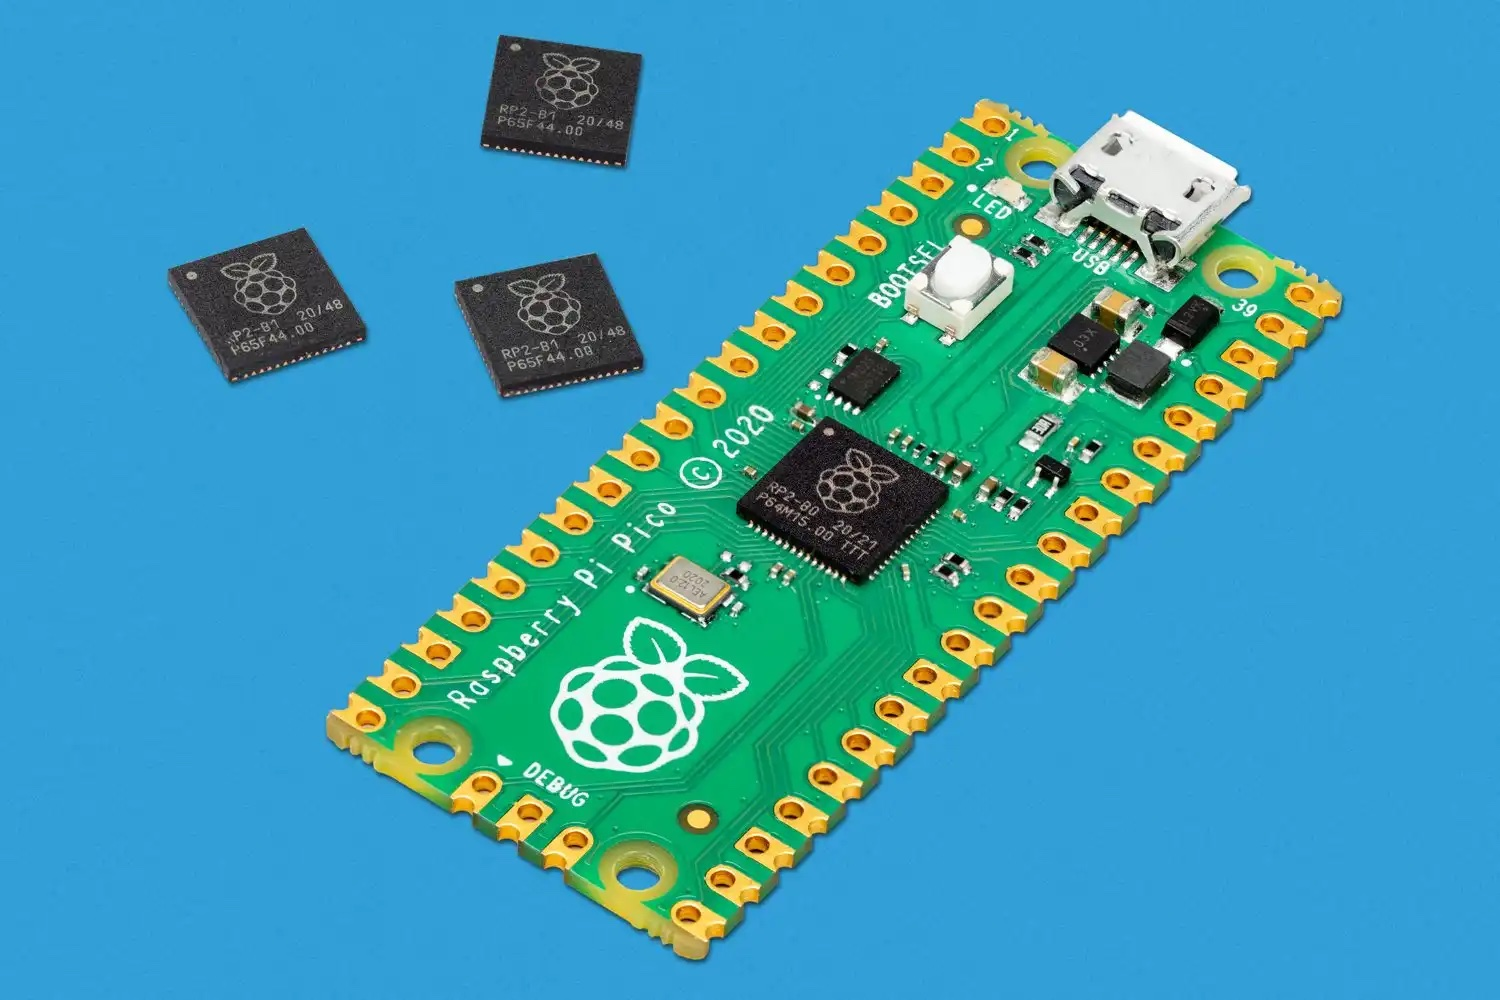
\includegraphics[width=\textwidth]{pico-rp2040}}
	\caption{Stock photo of Raspberry Pi Pico\cite{ltdBuyRaspberryPi}}
	\label{fig:picostock}
\end{figure}

The principle target recovery baord and project board are both a Raspberry Pi Pico \autoref{fig:picostock} which is a compact \gls{mcu} development platform created by the Raspberry Pi Foundation, running a dual core \gls{arm} Cortex M0 at 133Mhz with a larger than typical 264kB inbuilt \gls{ram} and 2MB of \gls{spi} flash memory storage for the class of \gls{mcu}\cite{ltdBuyRaspberryPi}.

The Pi Pico is relatively unusual for a \gls{mcu} in not containing any internal program execution flash memory, with programs executing either directly from RAM with boot time wait and upload, or more commonly directly out of attached \gls{qspi} flash with \gls{xip} functionality. External flash access is inherently much slower than normal internal programmable ROM flash due to the \gls{spi} bus, but to aid in achieving near equivalent execution speed the Pico has a configurable \gls{xip} hardware module that by default utilises 16kB of it's internal RAM as a cache for code execution, which is automatically maintained by the hardware. This \gls{xip} design is one of the ways the price of the Pi Pico is kept low, as only one silicon package design is needed unlike typical \gls{mcu}'s that come in a variety of configurations with different flash package sizes depending upon need, whilst also allowing much larger storage sizes without complicating software design as the full external \gls{spi} flash is mapped directly into address space by the inbuilt ROM library.

%TODO: Why not talk about pico XIP? Executing code directly out of SPI flash is quite unique concept  DONE

%The Pico is capable of having it's software image programmed to it via inbuilt ROM USB flasher using a UF2 image or via \gls{swd} interface.

\clearpage
\subsection{Pico Display Pack}
A Pimoroni Pico DIsplay Pack\autoref{fig:picodisplaypack} was selected as the user interface hardware for development due to availability on hand, but is a non critical component that could be swapped for other displays and input with relatively minor adjustment.

The Display Pack features four tactile buttons and a 1.14” 240x135 pixel IPS LCD screen to allow user feedback and input in order to allow a feedback interface for following progress in a more user friendly manner than something akin to a set of simple status LED's which would be hard to intuitively interpret.

\begin{figure}[ht]
	\centering
	\AltText{Stock photo of Pimoroni Pico DIsplay Pack}{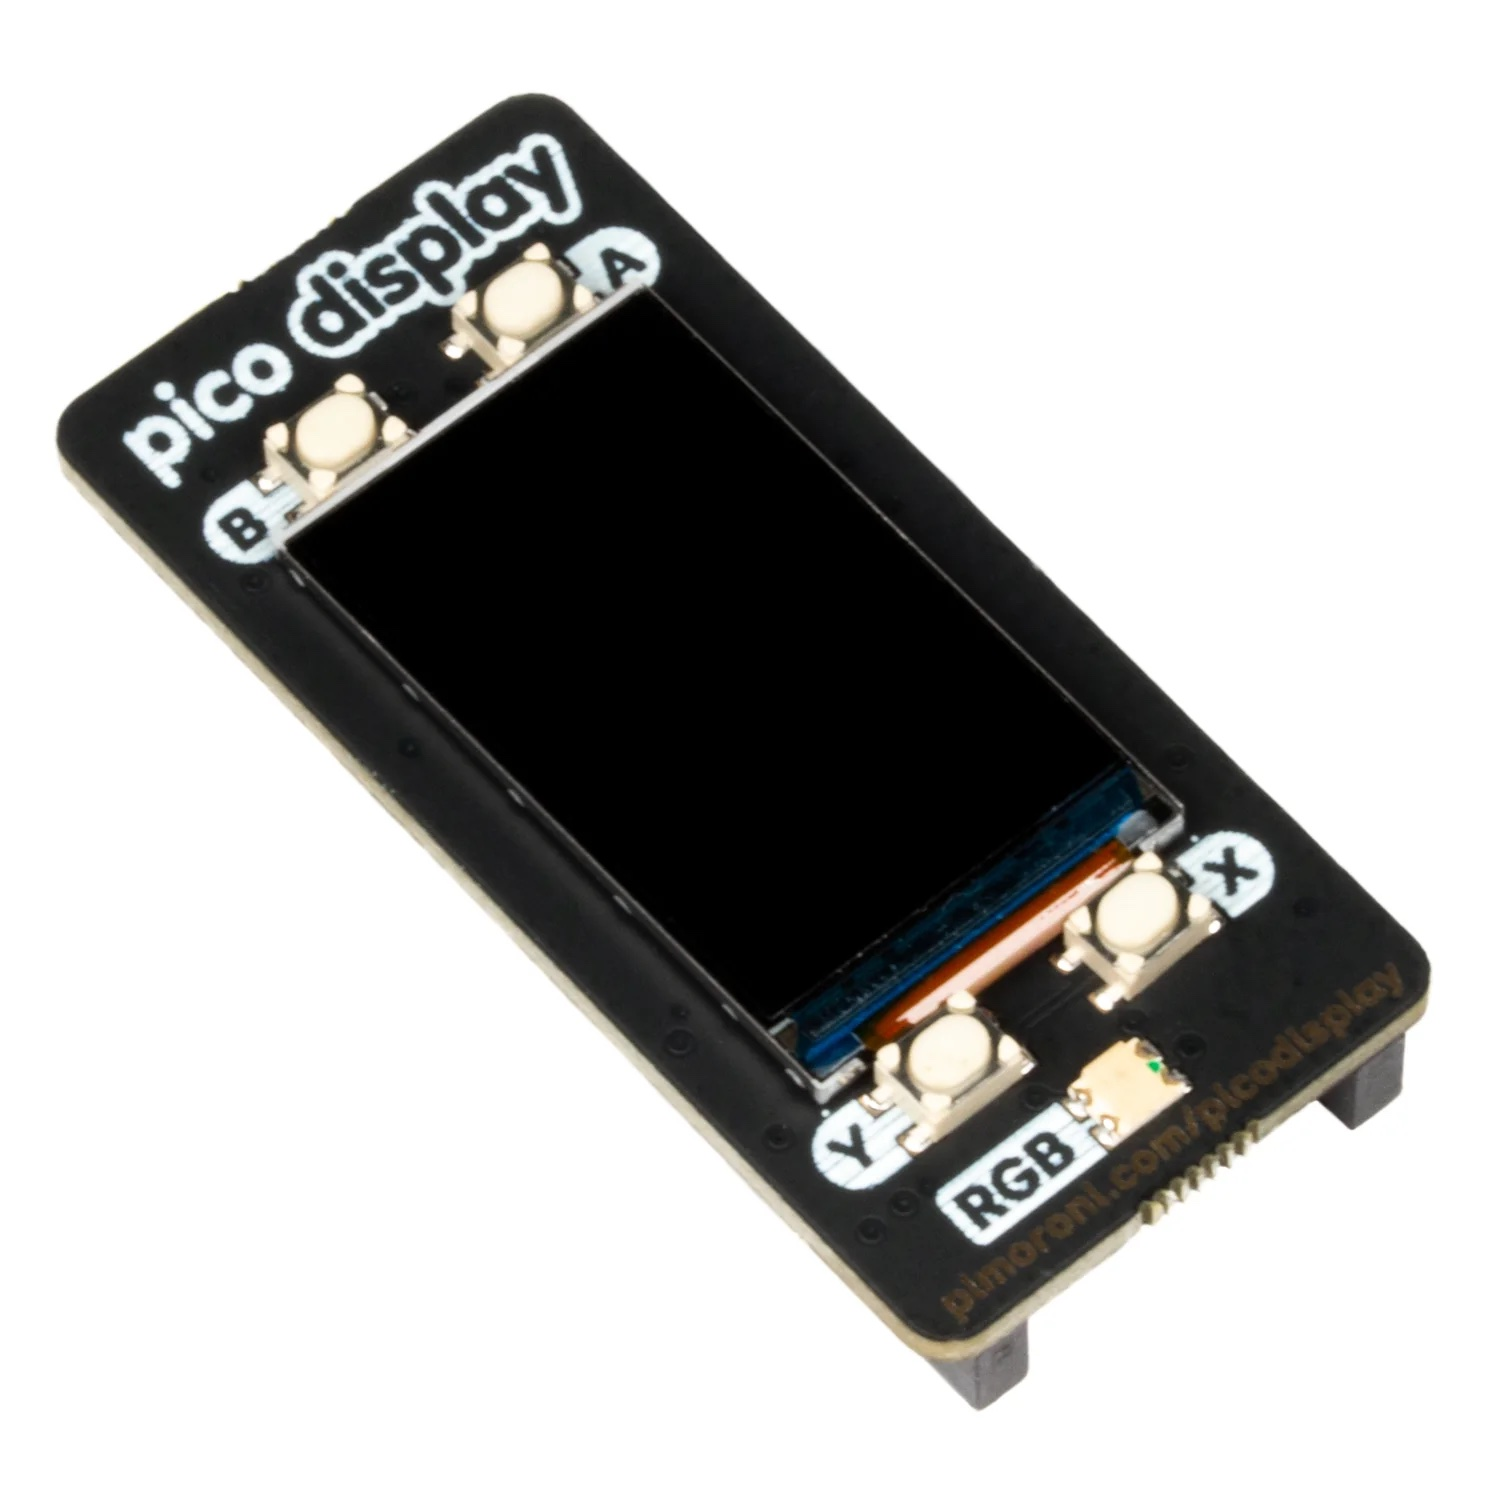
\includegraphics[width=.66\textwidth]{picodisplaypack}}
	\caption{Stock photo of Pimoroni Pico DIsplay Pack\cite{PicoDisplayPack}}
	\label{fig:picodisplaypack}
\end{figure}
	
\clearpage
\subsection{J-Link EDU Mini}
For debugging and rapid prototyping a J-Link EDU Mini\cite{JLinkEDUMini}\autoref{fig:jlinkedumini} from SEGGER GmbH was used as the hardware debugger for project to enable rapid development and debugging without constant manual image upload cycles during testing.

This is a \gls{usb} compact hardware debugger for embedded platforms to provide direct flashing and debug access to the Pi Pico to provide a more convenient development environment with one click compiling and target flashing, and allows utilisation of SEGGER's RTT library for debug messaging output and debug testing commands with low impact to operational performance and no extraneous hardware interfaces.

\begin{figure}[ht]
	\centering
	\AltText{Stock photo of J-Link EDU Mini}{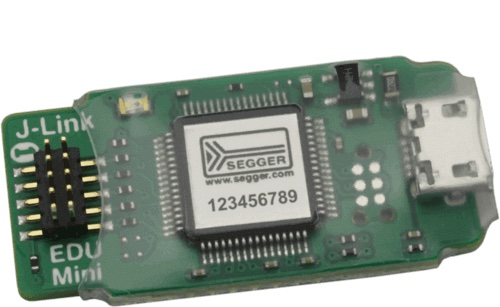
\includegraphics[width=.66\textwidth]{jlinkedumini}}
	\caption{Stock photo of J-Link EDU mini\cite{JLinkEDUMini}}
	\label{fig:jlinkedumini}
\end{figure}

\clearpage
\section{Ways to access Raspberry Pi Pico flash}

There are a couple of potential ways to be able to access the flash memory on the pico to be able to alter or reflash it as desired, with the most common and usually used method for uploading software images performed by holding down the 'BOOTSEL' button when plugging the Pi into \gls{usb}, which disabled the \gls{qspi} flash memory chip select line temporarily during boot process and causes the \gls{mcu} to automatically go into flashing mode whereupon the chip presents a virtual fat drive as a mass storage device to the \gls{usb} host allowing an image to be dragged on and flashed.

Whilst there is a standard \gls{spi} protocol for accessing flash modules, this is limited to 24 bit addressing over a single \gls{spi} lane which limits default \gls{rom} access to a maximum of 16 Megabytes at slow speeds. In order to allow larger module sizes and faster operation speeds \gls{qspi} is supported, which allows 4 bit parallel data transfer for fast operation, but due to lack of standardisation for initialising and accessing these modules in full address space and speed custom initialisation code is needed per device.

In order to allow the inbuilt hardcoded Pi Pico \gls{rom} bootloader to be able to run code directly via \gls{xip} on any possible \gls{spi} module, current or future without limitations, a small secondary bootloader called boot2 is required to be placed at the start of the flash module which is loaded by the \gls{rom} bootloader using standard SPI protocols. This boot2 image is responsible for initialising the specific module to which software image has been targetted and starting final program execution, and is normally managed by the Pico SDK project setup where flash type is specified.

%TODO You should also describe the normal bootloading process and what options you have there. There is a secondary bootloader (or config) on the flash... Done

This method could be used to run a \gls{ram} resident program via specific UF2 loading addresses which could be used to examine the flash memory and run an automatic recovery of a filesystem from MicroPython without affecting the primary flashed application.

But this method is cumbersome, as it cannot be fully automated due to the requirement of manual BOOTSEL enablement to enable whilst plugging in. There are ways to enter recovery mode without pressing BOOTSEL via \gls{usb} interface using picotool application that can make negotiate a pico running firmwares based on standard \gls{usb} stack to reboot into recovery mode\cite{picotool}, but this is inflexible and would not help recovering an application that immediately disables USB automatically at boot which is one of the primary requirements of the project.

The other principle method of being able to arbitrarily access flash memory on pico is via the \gls{arm} \gls{swd} debug interface using the board accessible debug pads intended for direct programming and onchip debugging\cite{ARMDebugInterface}.

The \gls{swd} interface  is always available regardless of firmware setup, and allows full control of the chip thus making it possible to fully automate. The principle disadvantage of this approach is the less convenient physical access to the interface compared to connecting to a \gls{usb} host.
\clearpage
\section{SWD interface}
The \gls{arm} \gls{swd} interface is an \gls{arm} microdevices created standard for all \gls{arm} Cortex CPU's using two wires for clock and signal, that allows bidirectional communication over a single signal wire and a variable host controlled signal speed.

Typical \gls{swd} control speeds range from 4-25MHz clock, though to achieve high clock rates typically seperate hardware such an \gls{fpga} programmed for dedicated signal control is used. Bue due to the debugger controlled clock, timing is not critical and can be flexible allowing a more simplistic 'bit banging' approach to be used from any GPIO interface, though more refined methods utilising peripheral hardware inside an \gls{mcu} can be possible, such as \gls{spi} controller, or in the case of the Pi Pico there is a relatively unique {\gls{pio} hardware interface that can be utilised for \gls{swd} as utilised in the Raspberry Pi Foundations Pi Pico based debug probe.

\gls{pio} is in effect a pair of smaller very simple tertiary sub processor modules on the pico that run state machines dedicated to \gls{gpio} processing. \gls{pio} state machines are written using a proprietary Assembly language that allow custom protocols to be implemented in a flexible way with tight hardware timing without the inconvenience of processor interrupts. That makes achieving such processing with a tightly controlled timing almost impossible with software controlled \gls{gpio} outside all but the simplest control systems.

%TODO  Maybe a few words about pio assembly here? DONE

Communication with the debug unit is first established with a reset sequence, which will always reset the debug unit to a known starting state so that connection can be established regardless of existing state.

Every transaction consists of a multiple phase process. First a request header to signal read or write a register including contained command validation parity check is clocked out onto the \gls{swd} I/O line, after which the host switches to reading the I/O line and clocks in three bits to check for an acknowledgement reply indicating whether the request was received, debug unit is busy or can action the request, or if the debug unit is in fault state.

If the acknowledgement is an all OK, then the next action is either clocking in the bus for length of data to read response, or switching back to clocking out the transmitted data packet. In the case of \gls{ap} memory reads, the first data read after a initial read request has to be ignored and discarded to give the debug unit time to retrieve the memory data, thus read cycle will always have an extra throwaway read at the end also.

After a data transfer if no other command is to be immediately processed an extra 8 clock cycle idle has to be continued post transfer to allow the debug unit to process requests internally such as memory writes. This ensures that the debugger is not left in an unknown state of execution which could result in unexpected behaviour.

\begin{figure}[ht]
	\centering
	\AltText{Diagram of ARM SWD memory write operation}{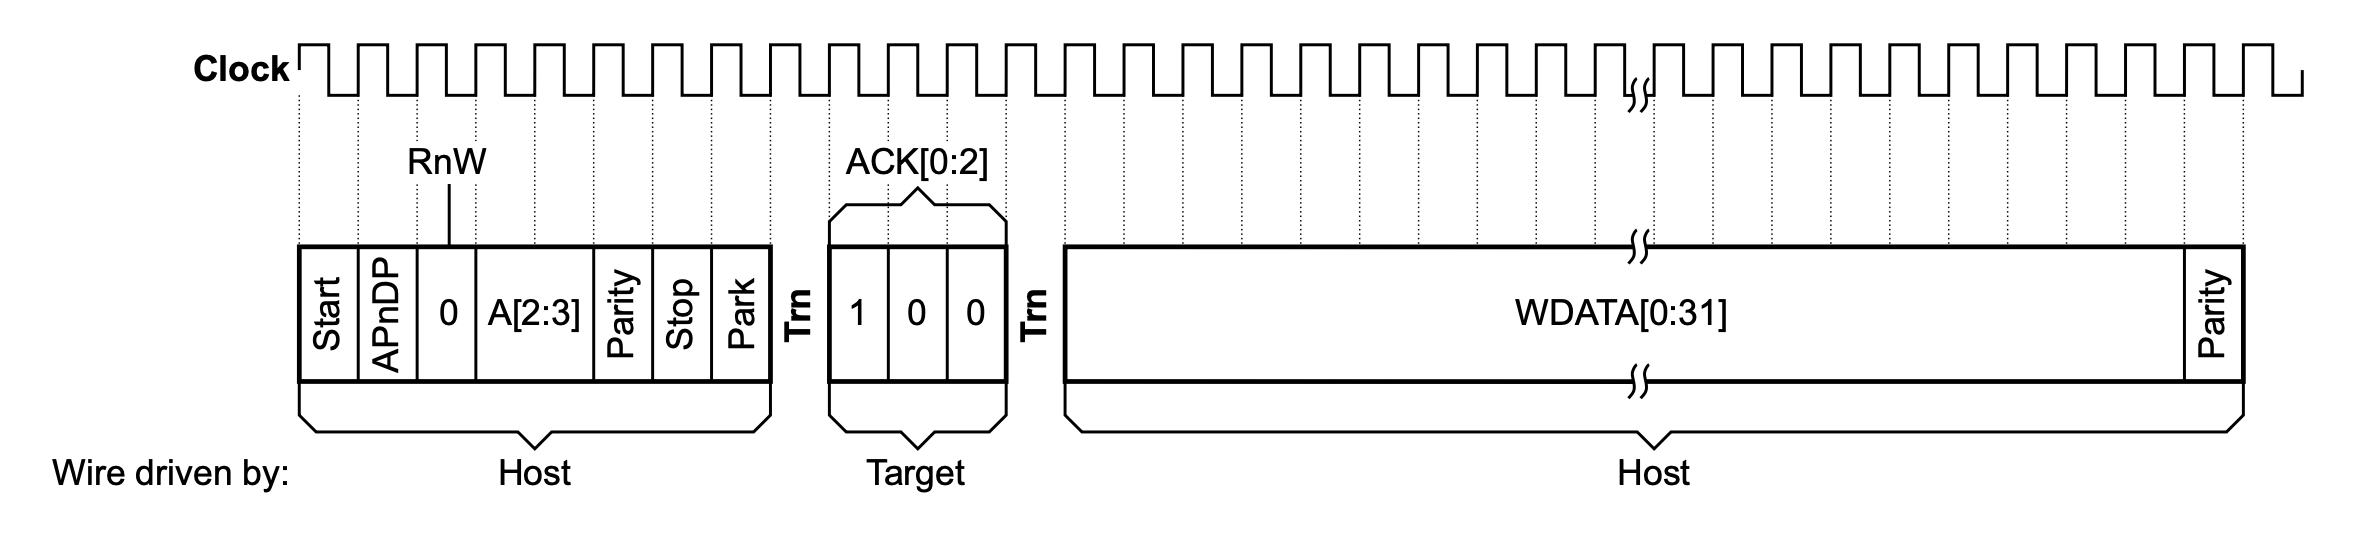
\includegraphics[width=\textwidth]{armswdwrite}}
	\caption{Diagram of SWD memory write\cite{ARMDebugInterface}}
	\label{fig:armswdwrite}
\end{figure}

\gls{arm} \gls{mcu}'s can also optionally support \gls{jtag} protocol debugging, using the same pins as \gls{swd}. For chips supporting both a handshake to establish the protocol being used is needed. But as the Pico is an \gls{swd} only \gls{mcu}, this part of the connection protocol is not needed which simplifies initialisation for the target device.

Each CPU core has it's own debug unit, along with a third 'reset' unit that can be used to reset the whole \gls{mcu}, and \gls{swd} control allows commanding the debug units in the \gls{mcu}, which allows reading and writeing memory, control of execution including setting breakpoints and other debug aiding measures.

\gls{swd} cannot directly access the flash memory on the Pico as this is external to the \gls{cpu}, and in order to perform operations on flash memory via debug interface the \gls{mcu} has to be instructed in some manner using memory access and process control to perform the operations required indirectly. This can be done via direct instructions to perform required actions which are first written into memory whilst core is halted or waiting before a jump and execute is instructed step by step for direct flash programming, though this would be very inefficient due to amount of waiting for writes and instructions to be prepared and waited for. A simpler and more reliable method which is typically used for flash programming via debuggers is uploading a small stub flash loader application with which the debugger communicates via a defined shared memory space, where some form of flashing cache buffer can be filled for the stub to continue programming.

For controlling the \gls{swd} interface there are two main possible methods to consider. Firstly so called 'bit banging' \gls{gpio} signals utilising \gls{arm} code to control signal lines via direct access which is effectively entirely non hardware dependant. Secondly using a \gls{pio} module in the Pico which would allow a lower level clock accurate control of \gls{gpio} on the device, an example implementation of which available in the official Raspberry Pi Pico debugger PicoProbe project\cite{Picoprobe2023}. It is also potentially possible to utilise \gls{spi} peripheral in order to perform \gls{swd} transactions, though this was deemed unnecessarily complicated to investigate as a potential solution compared to the main methods already discussed.\cite{OpenOCDRaspberryPi}.

Due to \gls{swd}'s use of host device clock signal and no tight timing requirements for it's operation, the simpler software based 'bit banging' was implemented as first proof of concept, which combined with running the pico clock at a technically overclocked but still stable 230 MHz operating speed allowed faster timing in a simple manner opposed to implementing a more complex pio based solution.

%TODO:  SW based or pio assembly?  DONE

\clearpage
\section{Helper Binary Image}
In order to perform operations on the target device in an efficient manner without directly writing instructions to target memory for every operation a secondary memory resident helper application image is needed, which is embedded within the recovery flasher's image and uploaded to the target device on initialisation. The helper application is responsible for performing the actual recovery processes on the target hardware, such as reporting target hardware type to the recovery board using a detection routine based on ADC3 readings from voltage regulator depending upon a \gls{gpio} pin state that differs between Pico and Pico Wireless\cite{IdentifyingPicoPicoW}, reading /writing flash image and performing file system accesses and modifications.

Flash access is done in the helper application by calling into inbuilt bootloader ROM library routines on the target Pico to perform inbuilt default \gls{spi} flash initialisation to map external flash into address space and enable default ROM flash write routines to be callable for write operations in the same compatible manner the inbuilt BOOTSEL flasher performs. Due to the access speed requirements of flashing being lower than execution and necessary software image file system being within the default 24 bit address area of standard \gls{spi} flash access, no further boot2 initialisation for full flash chip capability is needed, mirroring normal BOOTSEL flash image write process.

\clearpage
\section{USB Flashing Format}
\gls{uf2} is a file format created by Microsoft with the intention of having a simple universal file format for device firmware image updates, that is very easy to support with a minimal loader to manage the flashing on target device, intended primarily for use via a \gls{usb} supporting bootloader that presents a virtual file system to the operating system via standard \gls{usb} \gls{msc} protocol, so that special hardware and software is not needed for firmware updates.

A \gls{uf2} file is composed of a series of 512 byte blocks, each of which consists of an identifying header, payload, and a closing end magic number to verify receipt of complete blocks\autoref{table:uf2header}. The Payload can be upto 476 bytes, but typically only 256 bytes are actually used to in order to align with flash block write sizes, helping keep block addressing simple. This typical underutilisation of payload allocation leads to a notable percentage of wasted space within files but ensures that file system writes over virtual \gls{usb} \gls{msc} always contain complete blocks\cite{USBFlashingFormat2023} allowing capturing and writing data to flash without buffering multiple writes in normal usage which simplifies flasher design. 

The 32 byte header of each block contains necessary information to direct flashing process such as the payloads destination flash address in \gls{rom}, a family code to verify device type the image is meant for, the relative number of current block, and a total block count for complete image.

\gls{uf2} block header also contains a flag field which allow s further optional features in the format, including a checksum for the data and presence of family type instead of file size which is typically used instead of the default file size field, as family field is useful to help prevent incorrect firmware uploads to desce and complete firmware image size being calculable from the stored block count data and assumption of typical payload size. Checksum data is not typically used, and thus not needed to be implemented.

This is enough information for flashing software to know where to put each part of image as received, and keep track of progress in order to know full image has been received without an explicit end of transfer or blocks received out of order, which is key to being able to flash images via \gls{usb} \gls{msc} file system write.

The format was chosen by the Pi foundation as the native image format for the pico due to this simplicity of use, and the pico recovery bootloader presents a \gls{usb} mass storage virtual \gls{fat} file system from it's \gls{rom} stored 16kB alongside \gls{usb} stack and \gls{rom} callable routines for functionality including \gls{spi} flashrom writing. When reading in an image the bootloader uses the target address of the image to signify whether to load the data into ram for immediate execution, or to flash and execute from \gls{qspi}.

\begin{table}[h]
	\centering
	\caption{UF2 Format Block header\cite{USBFlashingFormat2023}}%IMPORTANT the caption must be before the tabular, so it will be on top of the table (there are other tricks to force it on top; but this one is straightforward).
	\vspace{-16.5pt}%time to time, spacing between caption and table can go too big...
	
	\begin{tabular}{|l|l|l|}
		\hline
		Offset	& Size &	Value\\ \hline
		0	& 4 &	First magic number, 0x0A324655 ("UF2\textbackslash n")\\ \hline
		4&	4&	Second magic number, 0x9E5D5157\\ \hline
		8	&4&	Flags\\ \hline
		12&	4	&Address in flash where the data should be written\\ \hline
		16&	4	&Number of bytes used in data (often 256)\\ \hline
		20&	4	&Sequential block number; starts at 0\\ \hline
		24&	4	&Total number of blocks in file\\ \hline
		28&	4	&File size or board family ID or zero\\ \hline
		32&	476&	Data, padded with zeros\\ \hline
		508&	4&	Final magic number, 0x0AB16F30\\ \hline

	\end{tabular}
	\label{table:uf2header}
\end{table}

\clearpage
\section{USB Virtual Filesystem}
Standalone \gls{swd} control is enough to be able to recover a file system or erase a board to rescue bootloader state, but in order to fully setup a Pico from scratch a flash image to program is needed. This image could be included into the program as a binary include, but this makes updating cumbersome requiring recompiling and uploading a new full binary image to the recovery Pico, which is typically achieved by setting the Pico into BOOTSEL recovery mode and flashing the new combined \gls{uf2} image on.

It was figured that a more convenient alternative would be for the device to manage it's own images, which also allows device to signal what firmware is installed to the user via filename, and due to the requirement to support both Pico original and wireless editions, two separate firmwares  images need to be maintained in order to be able to utilise a single recovery board.

The \gls{uf2} format was created for simplicity of flashing to hardware via a bootloader, and is quite wasteful internally in typical usage as also applied by the Pi Pico flash images, with each 256B block of target flash using a full 512B in the file to make addressing simple, but this wastefulness along with header data containing mostly static unchanging data, barring changing addressing data allows the possibility to generate this data using only a list of addresses per block and a single unified header. This allows the possibility to utilise a more efficient custom storage format to more efficiently utilise storage and allow a standard 2MB Pico enough space to save flash images for typical use cases for both models.

All the \gls{uf2} header data barring addresses can be calculated at run time, so only the addresses for each flash block are required to be stored in a header, empty flash does not waste image space, nor non payload areas of the original \gls{uf2} image, thus virtually

\clearpage
\section{MicroPython and Filesystem}
One of the primary goals of the project is to recover a non booting MicroPython installation on a Pico, this requires interfacing with the local file system in some way, which is automatically created by the MicroPython environment if not existing upon first execution. Default file names are used for automatic boot time execution of programs which allow the scriptable environment to be used both user interactively via \gls{repl} or in an embedded system manner to act as fixed usage device.

MicroPython as a project supports various different file systems such as FAT, but for the Pi Pico port the filesystem used is the open source littlefs filesystem\cite{MicroPythonProject2023}. The littlefs file system\cite{Littlefsproject} used here is designed specifically for \gls{mcu}'s, designed to be safe for use in environments where constant power is not guaranteed and data integrity is needed by using a copy on write methodology where all updates to files are performed on a dynamic copy of the data with file table only updated when commit is complete and file closed to allow automatic fallback to last good state on unexpected power loss.




% Project Specifications
\clearpage%if the chapter heading starts close to bottom of the page, force a line break and remove the vertical vspace
\vspace{21.5pt}
\chapter{Implementation}
\section{Software  setup}

First state of project was getting initial programming environment ready, consisting of rp2040 SDK, Arm GCC cross compiler and Visual Studio Code\autoref{fig:vscode} with plugins for debugging and managing the rp2040 CMAKE build process, and a j-link SWD debugger to program and debug on the \gls{mcu} more flexibly than \gls{usb} UF2 flash programming. A logic analyser was also used in initial phases to help monitor the debug traffic for verification of handshake operations till communication was established between boards.

\begin{figure}[ht]
	\centering
	\AltText{Project loaded into Visual Studio Code}{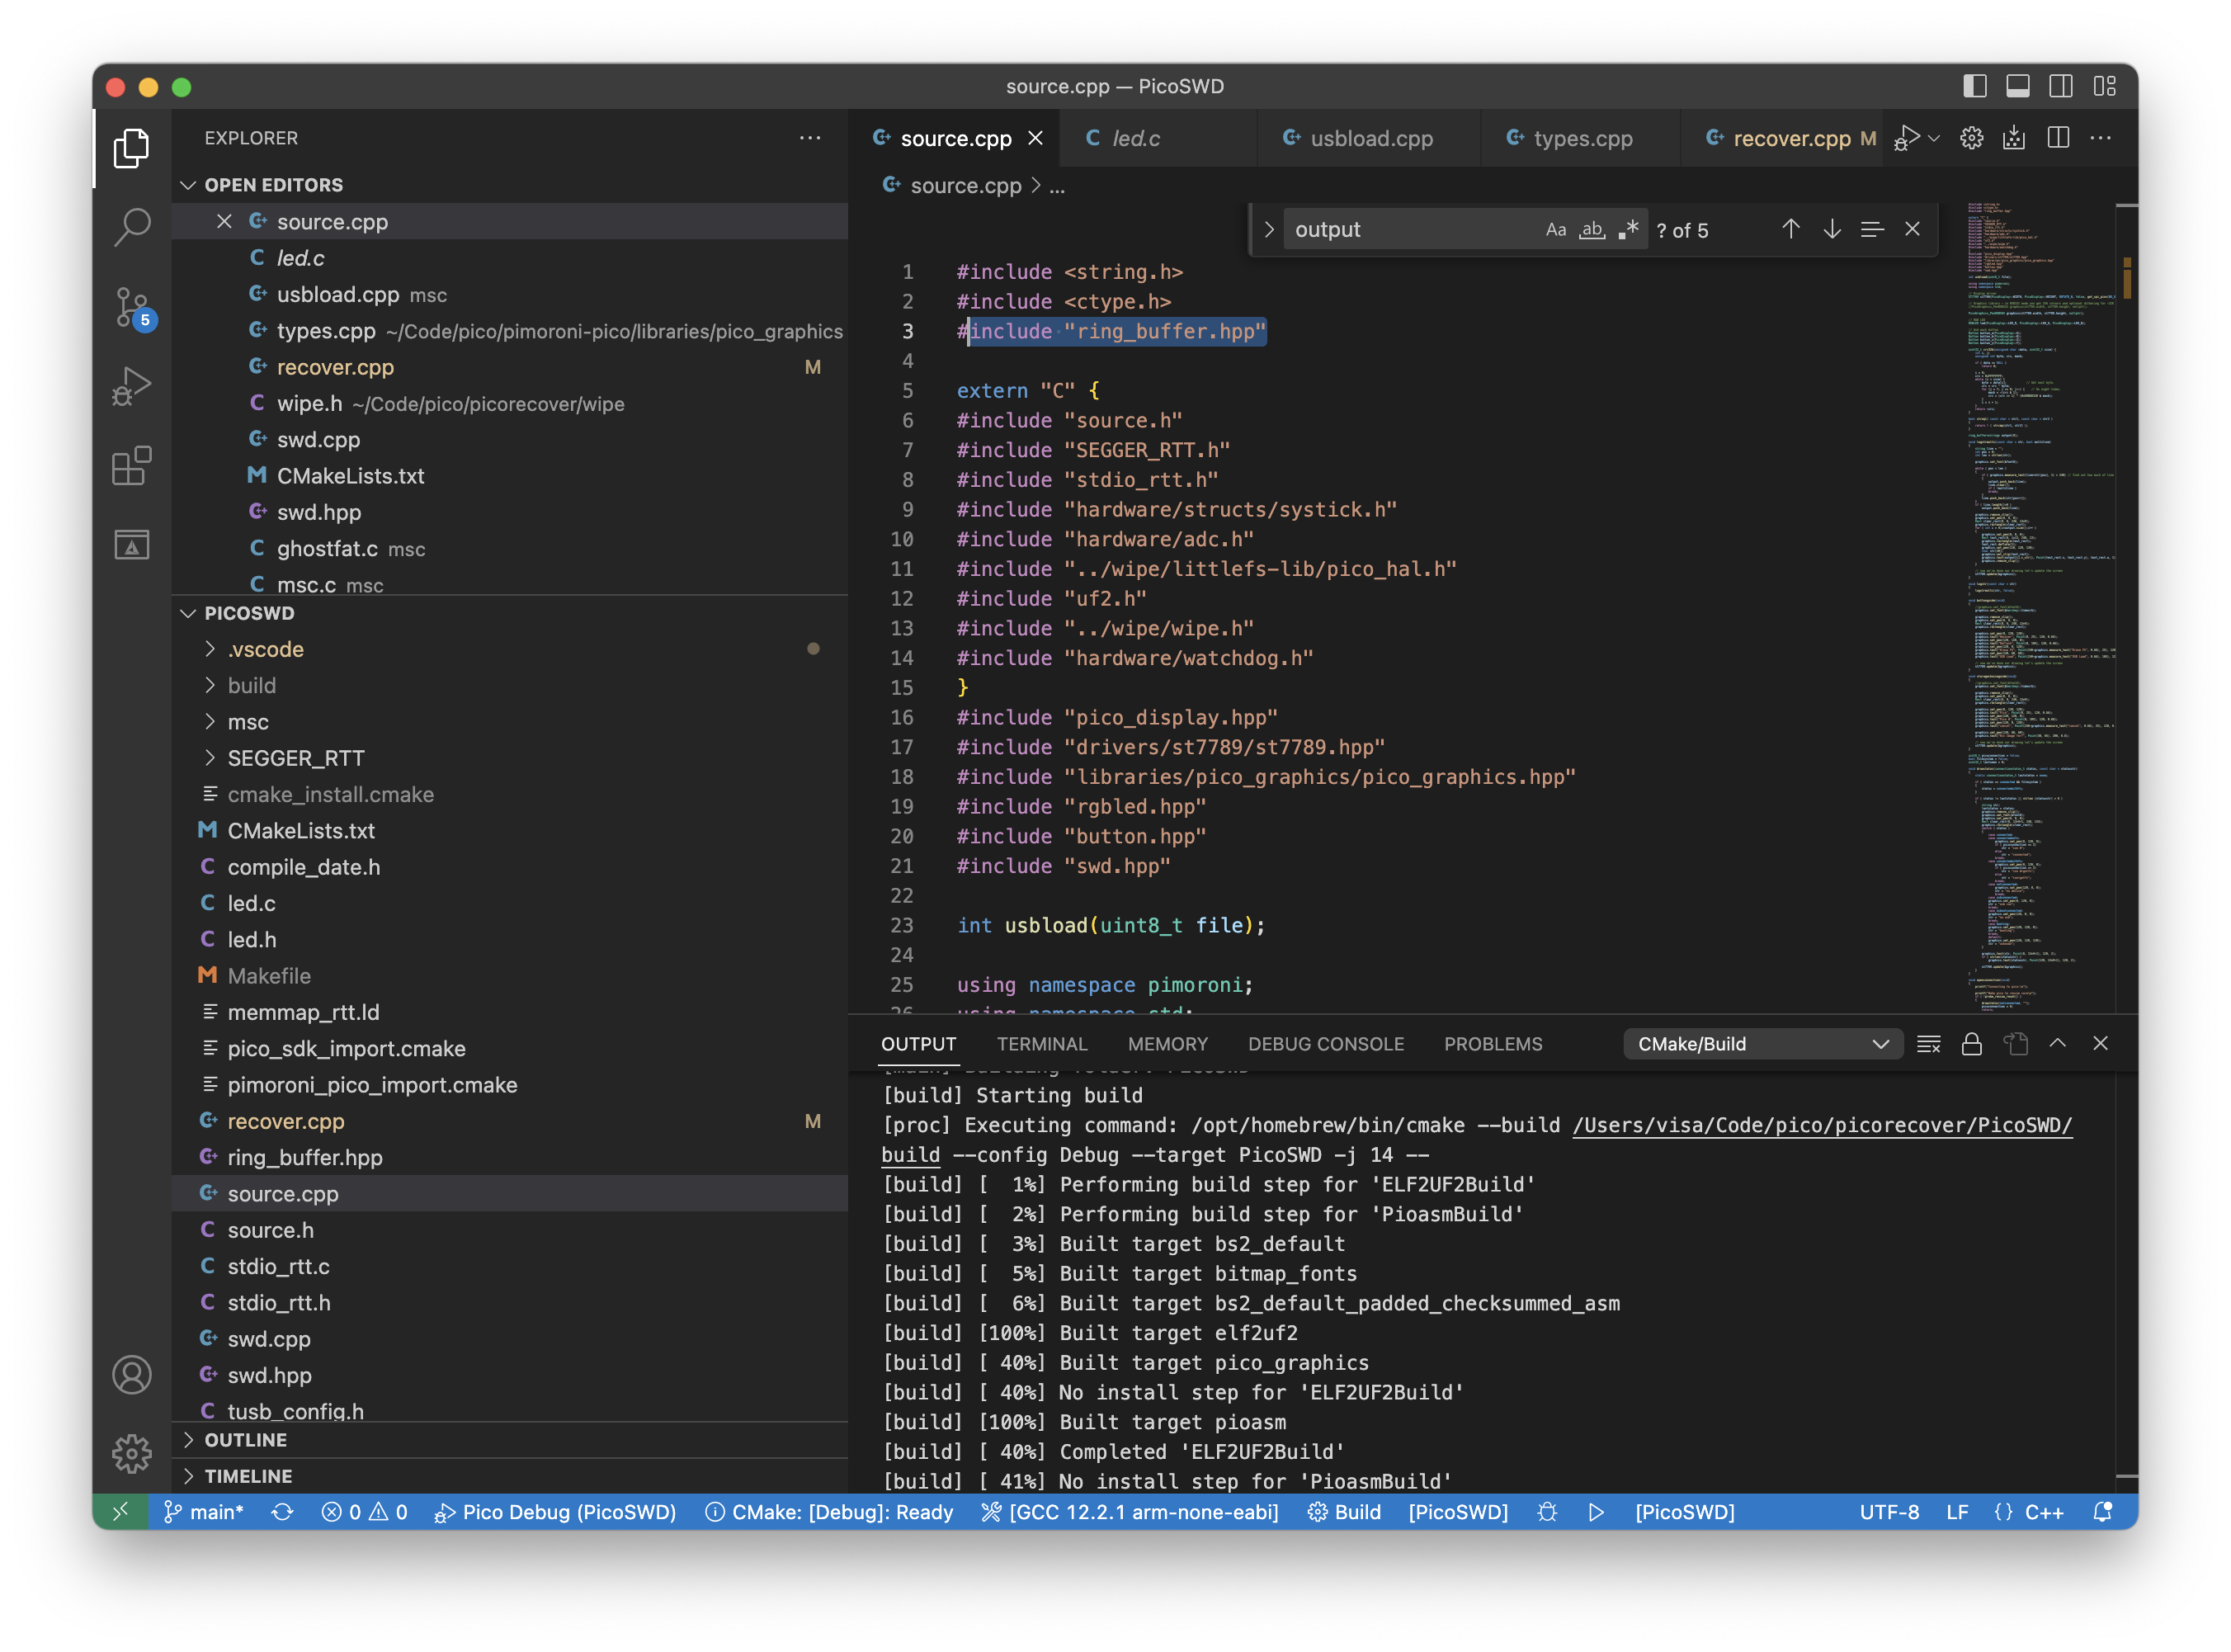
\includegraphics[width=\textwidth]{vscode}}
	\caption{Visual Studio Code}
	\label{fig:vscode}
\end{figure}

\clearpage
\section{Hardware setup}
%

For first testing of compilation environment as initial proof of concept test bench setup a Pi Pico was directly wired into a J-Link debugger for simplicity as show in \autoref{fig:InitialPOCwiring}.

\begin{figure}[ht]
	\centering
	\AltText{Initial proof of concept hardware setup showing direct soldered wiring between J-Link Edu and a Raspberry Pi Pico}{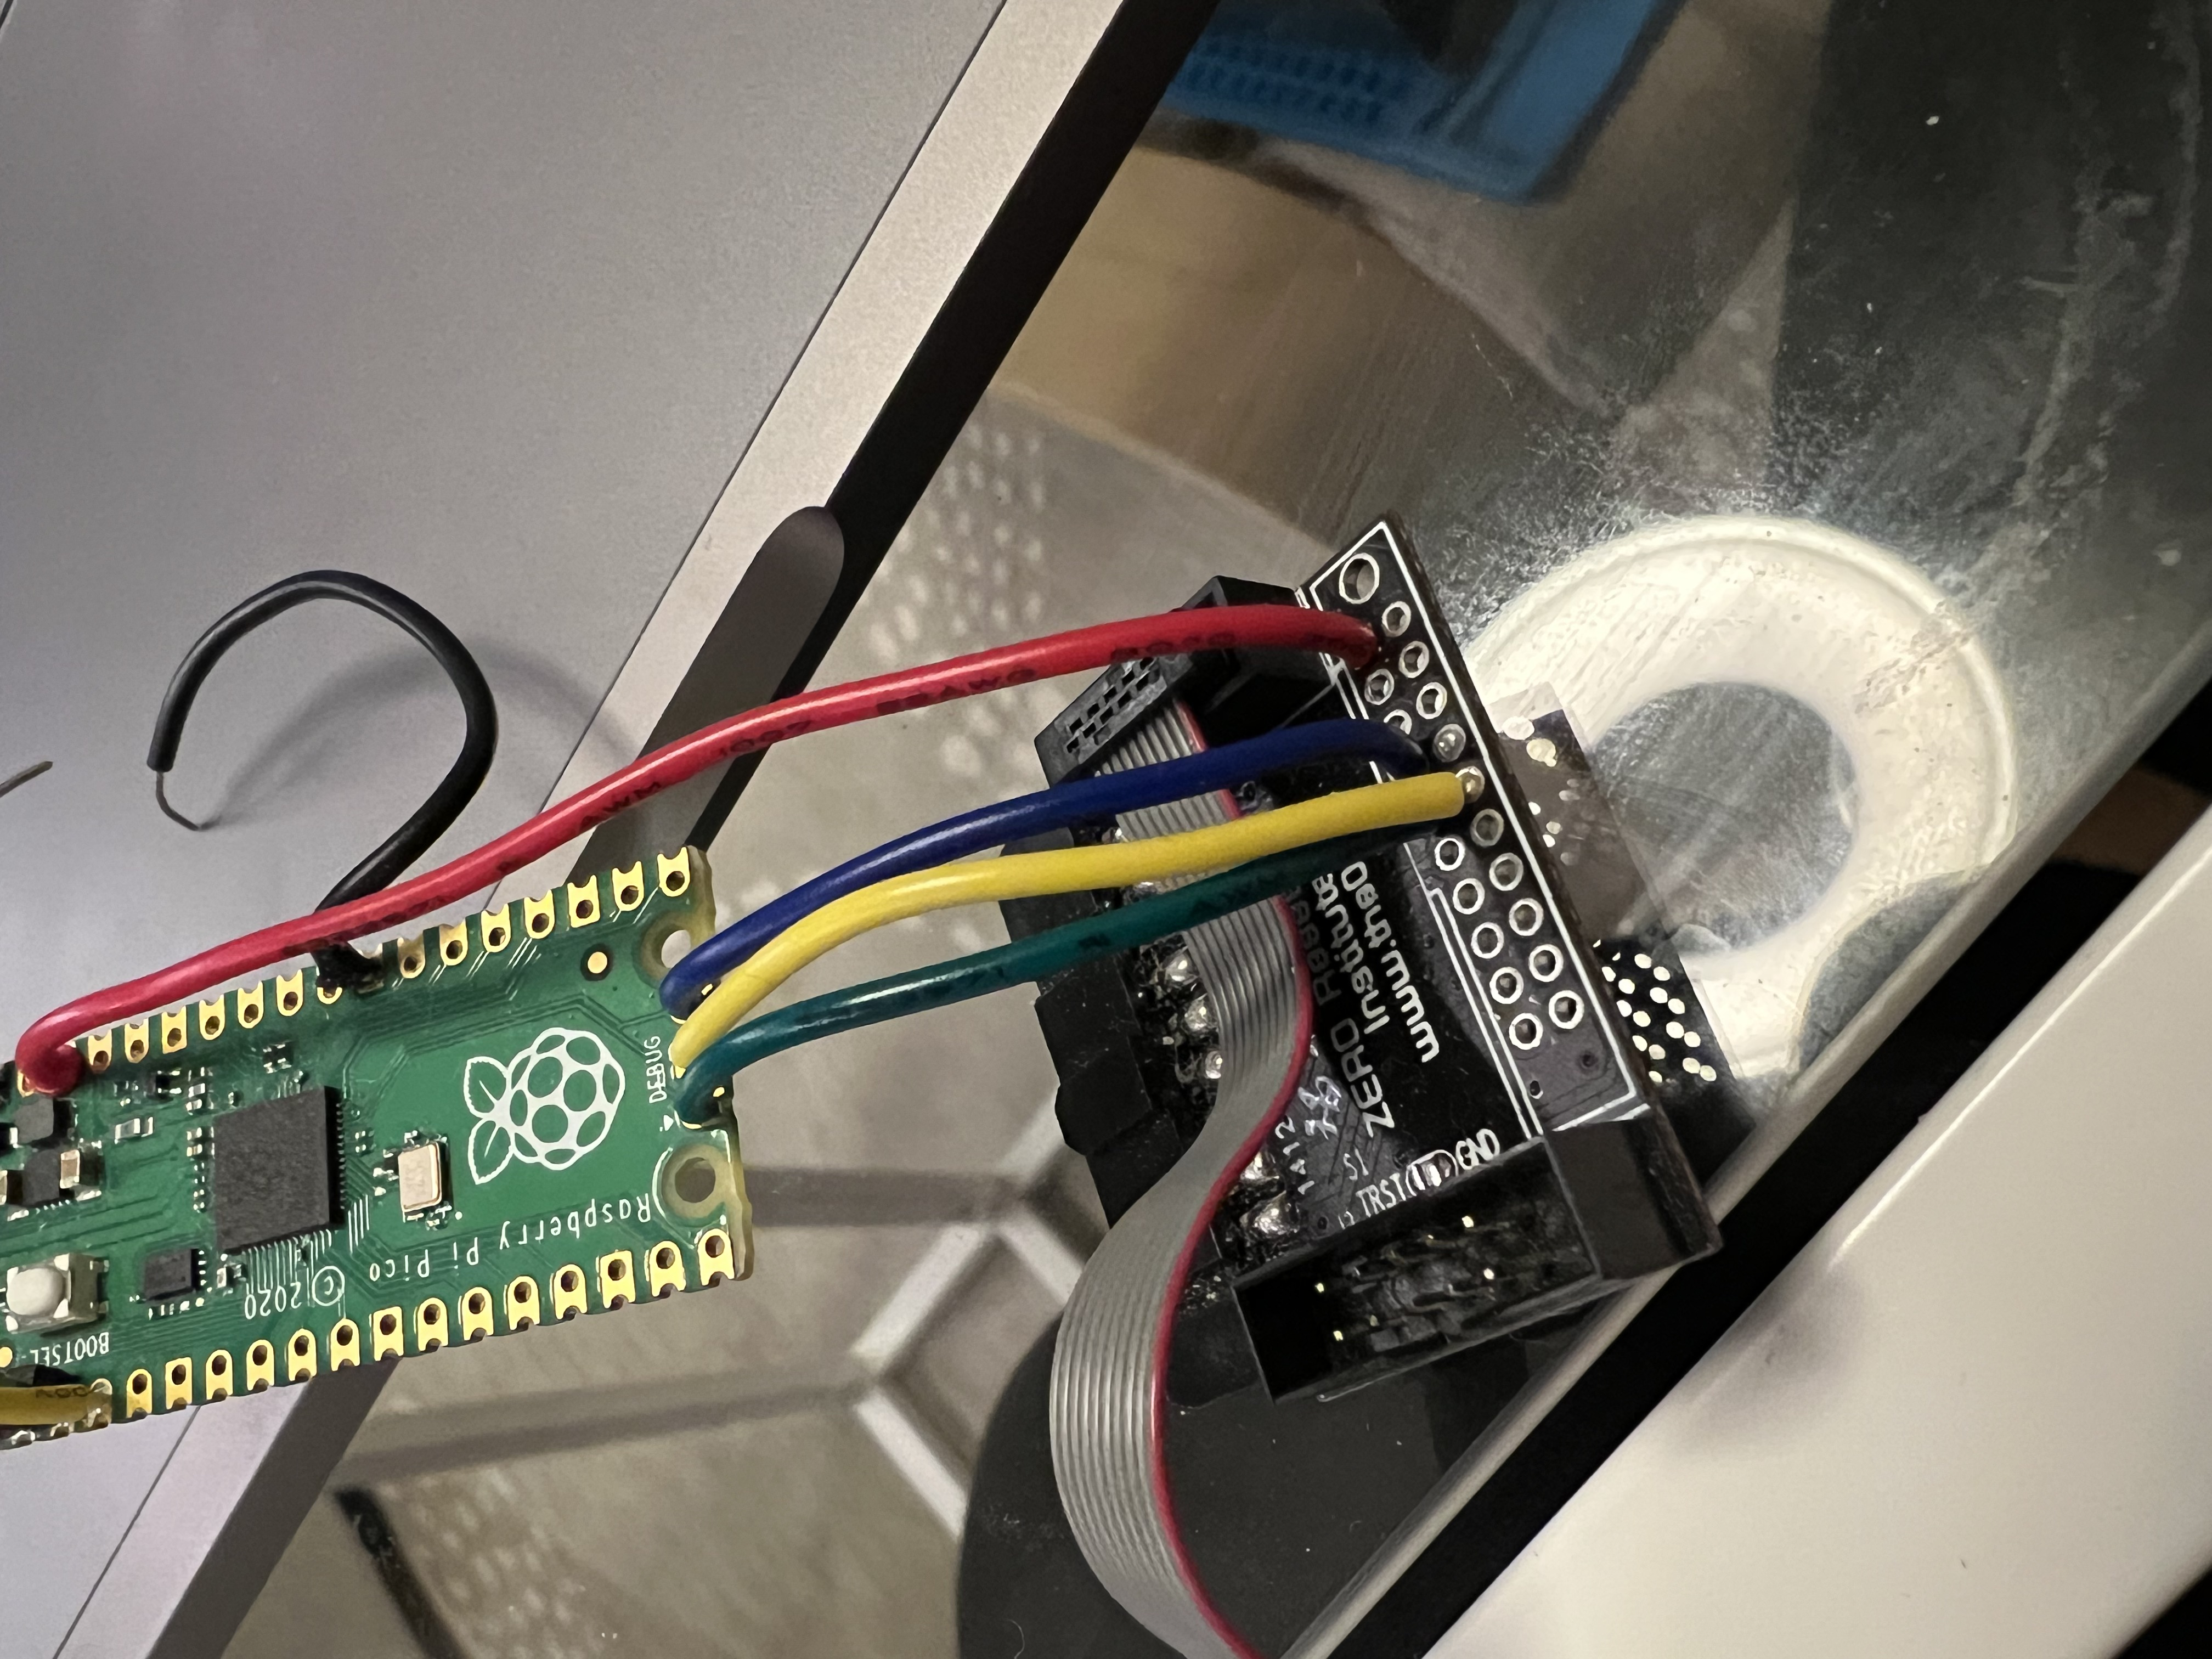
\includegraphics[width=\textwidth]{initial POC setup}}
	\caption{initial POC setup}
	\label{fig:InitialPOCwiring}
\end{figure}

Segger RTT library\cite{JLinkRTTReal} is used for debug console access during testing to eliminate need for a separate UART/Serial receiver and associated wiring, simplifying test setup considerably whilst allowing rapid interactive testing. 

This setup was further expanded upon to include the second Pi Pico target device and a removable interlock wire used to simulate the closing of a mounting interface interlock to enable simulating plugging and unplugging target board without physically removing all wiring between boards on bench setup whilst getting initial communication operable. Once essential functionality for performing recovery operations was implemented the hardware setup was further expanded to include a Pimoroni Display Pack to provide for an end a user interface beyond debug testing, and second Pi Pico as flashing target \autoref{fig:FullPOCwiring}, with wiring diagram as shown in \autoref{fig:FullPOCwiringDiagram}

\begin{figure}[ht]
	\centering
	\AltText{Full POC hardware setup showing display and buttons for UI on breadboads along with target device}{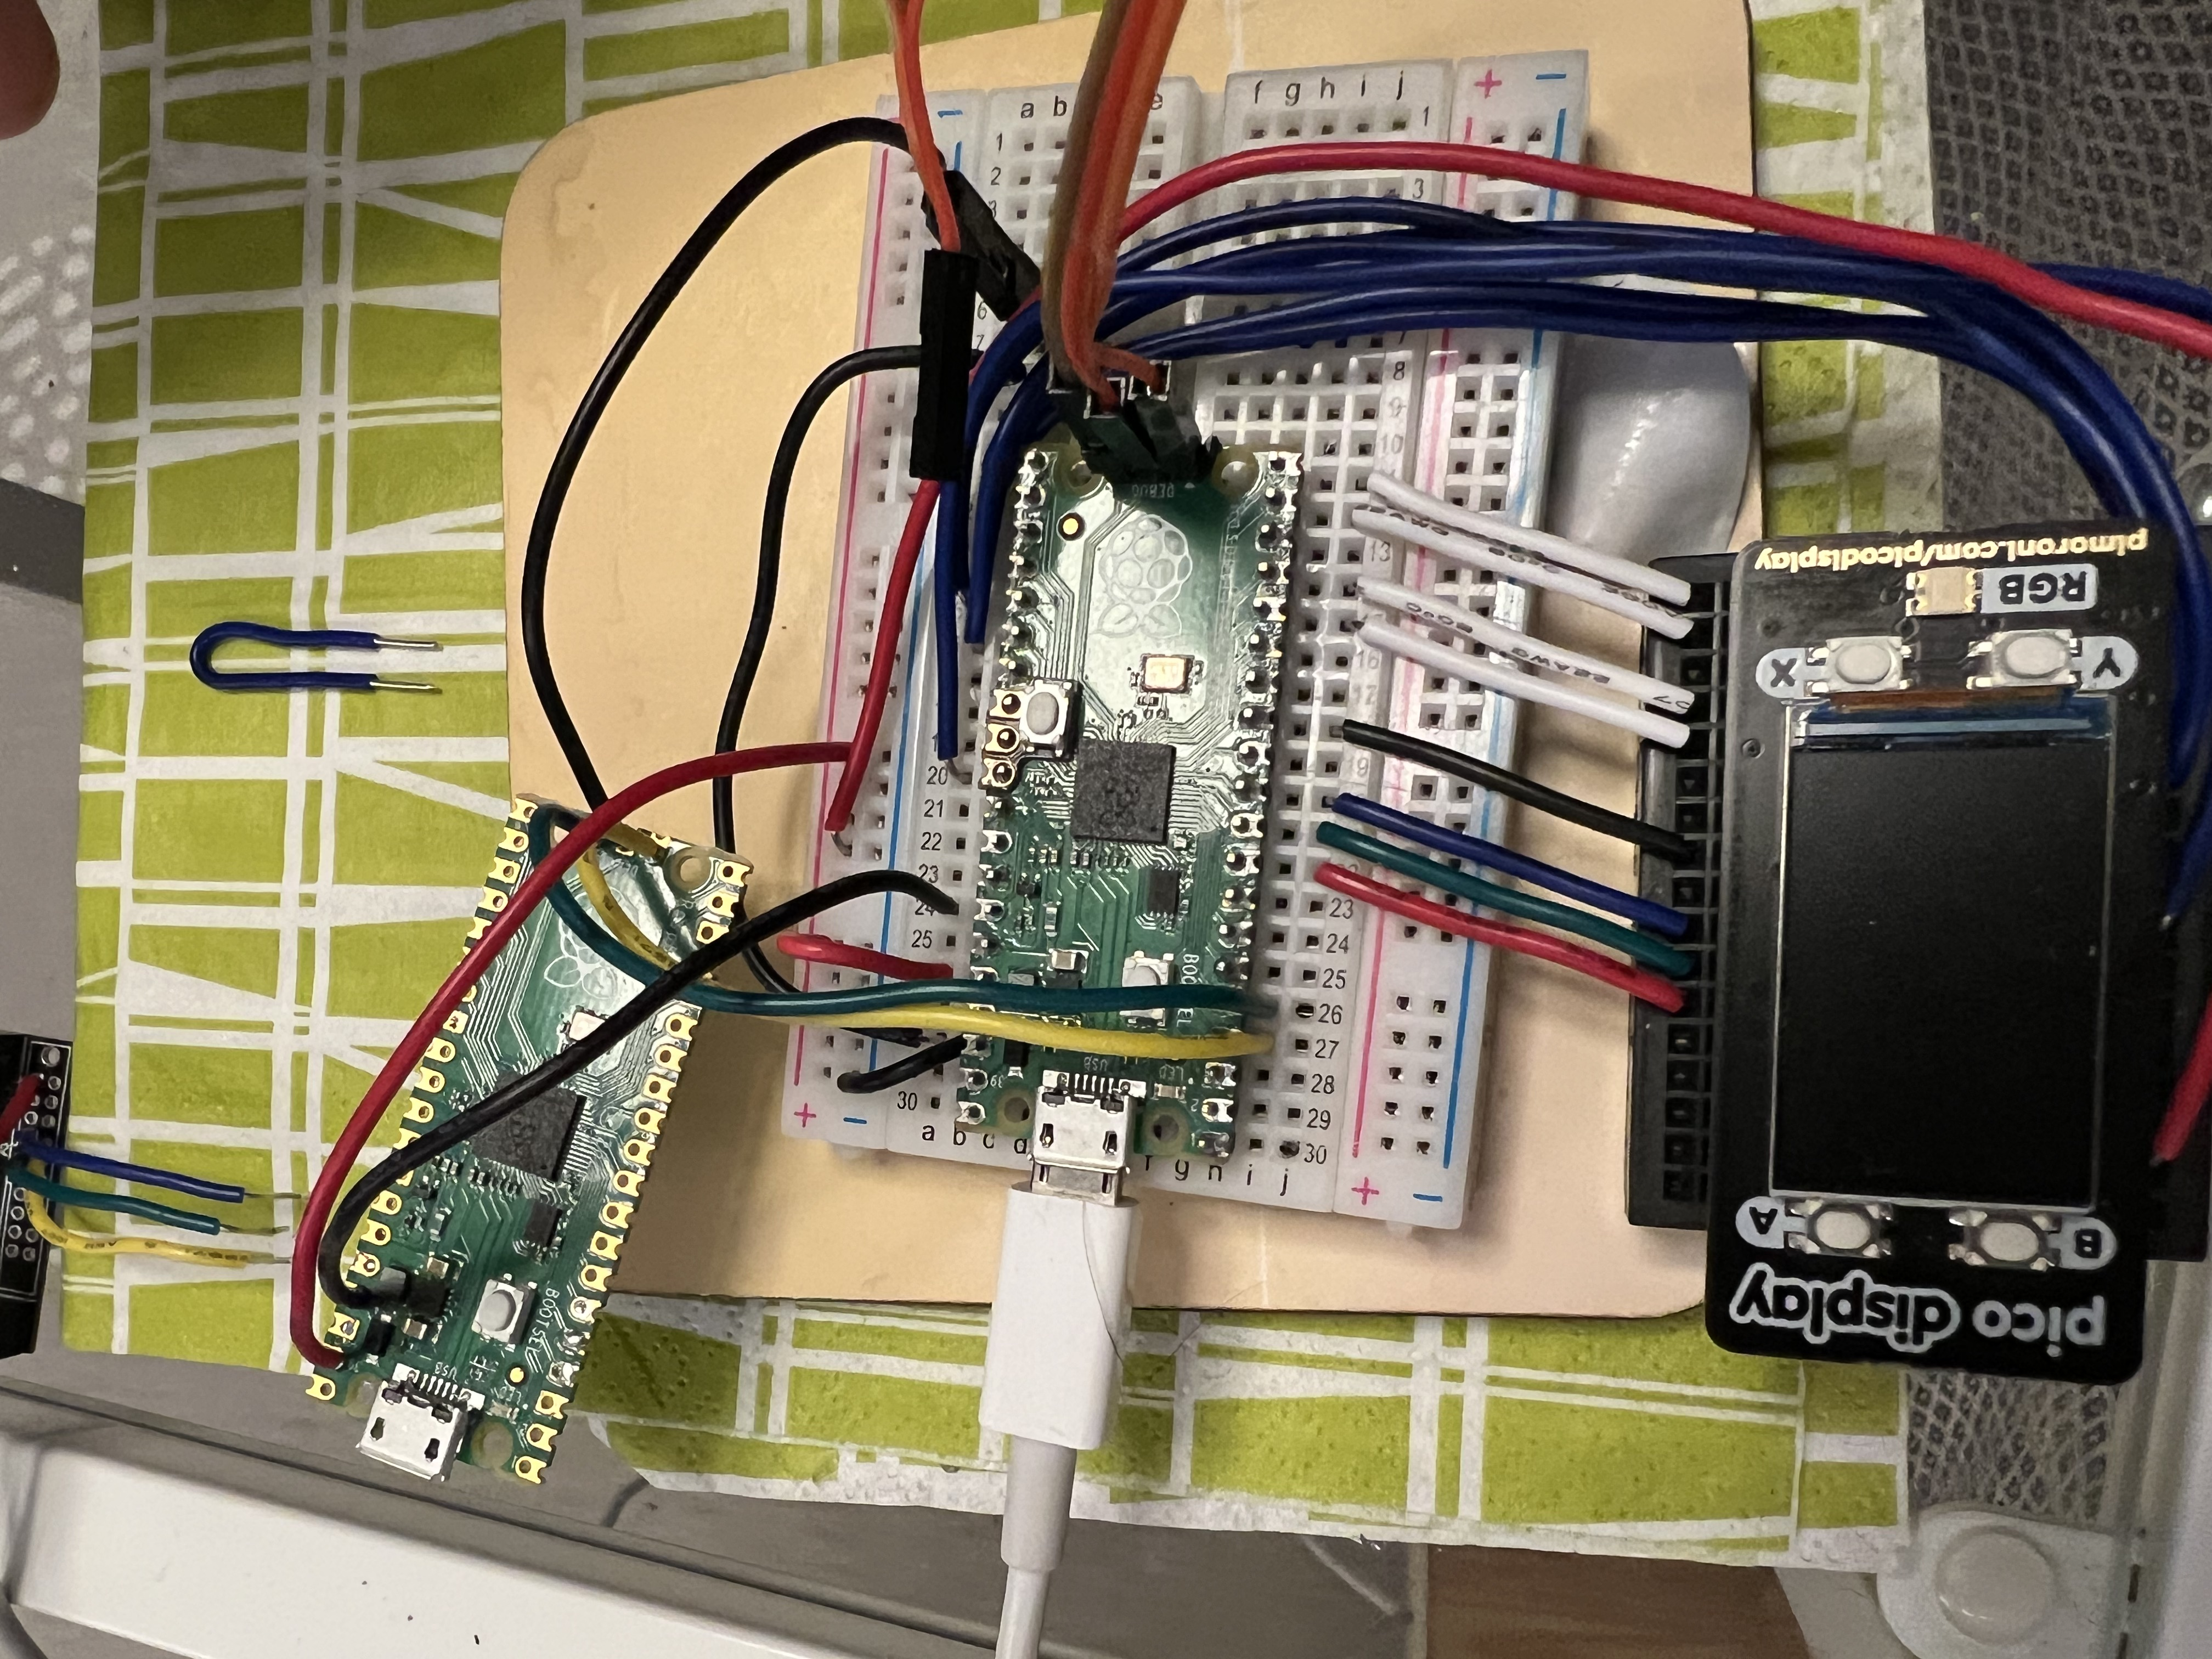
\includegraphics[width=\textwidth]{full POC setup}}
	\caption{Full wiring on breadboard with Interface}
	\label{fig:FullPOCwiring}
\end{figure}

\begin{figure}[ht]
	\centering
	\AltText{Ki-Cad wiring schematic of POC setup}{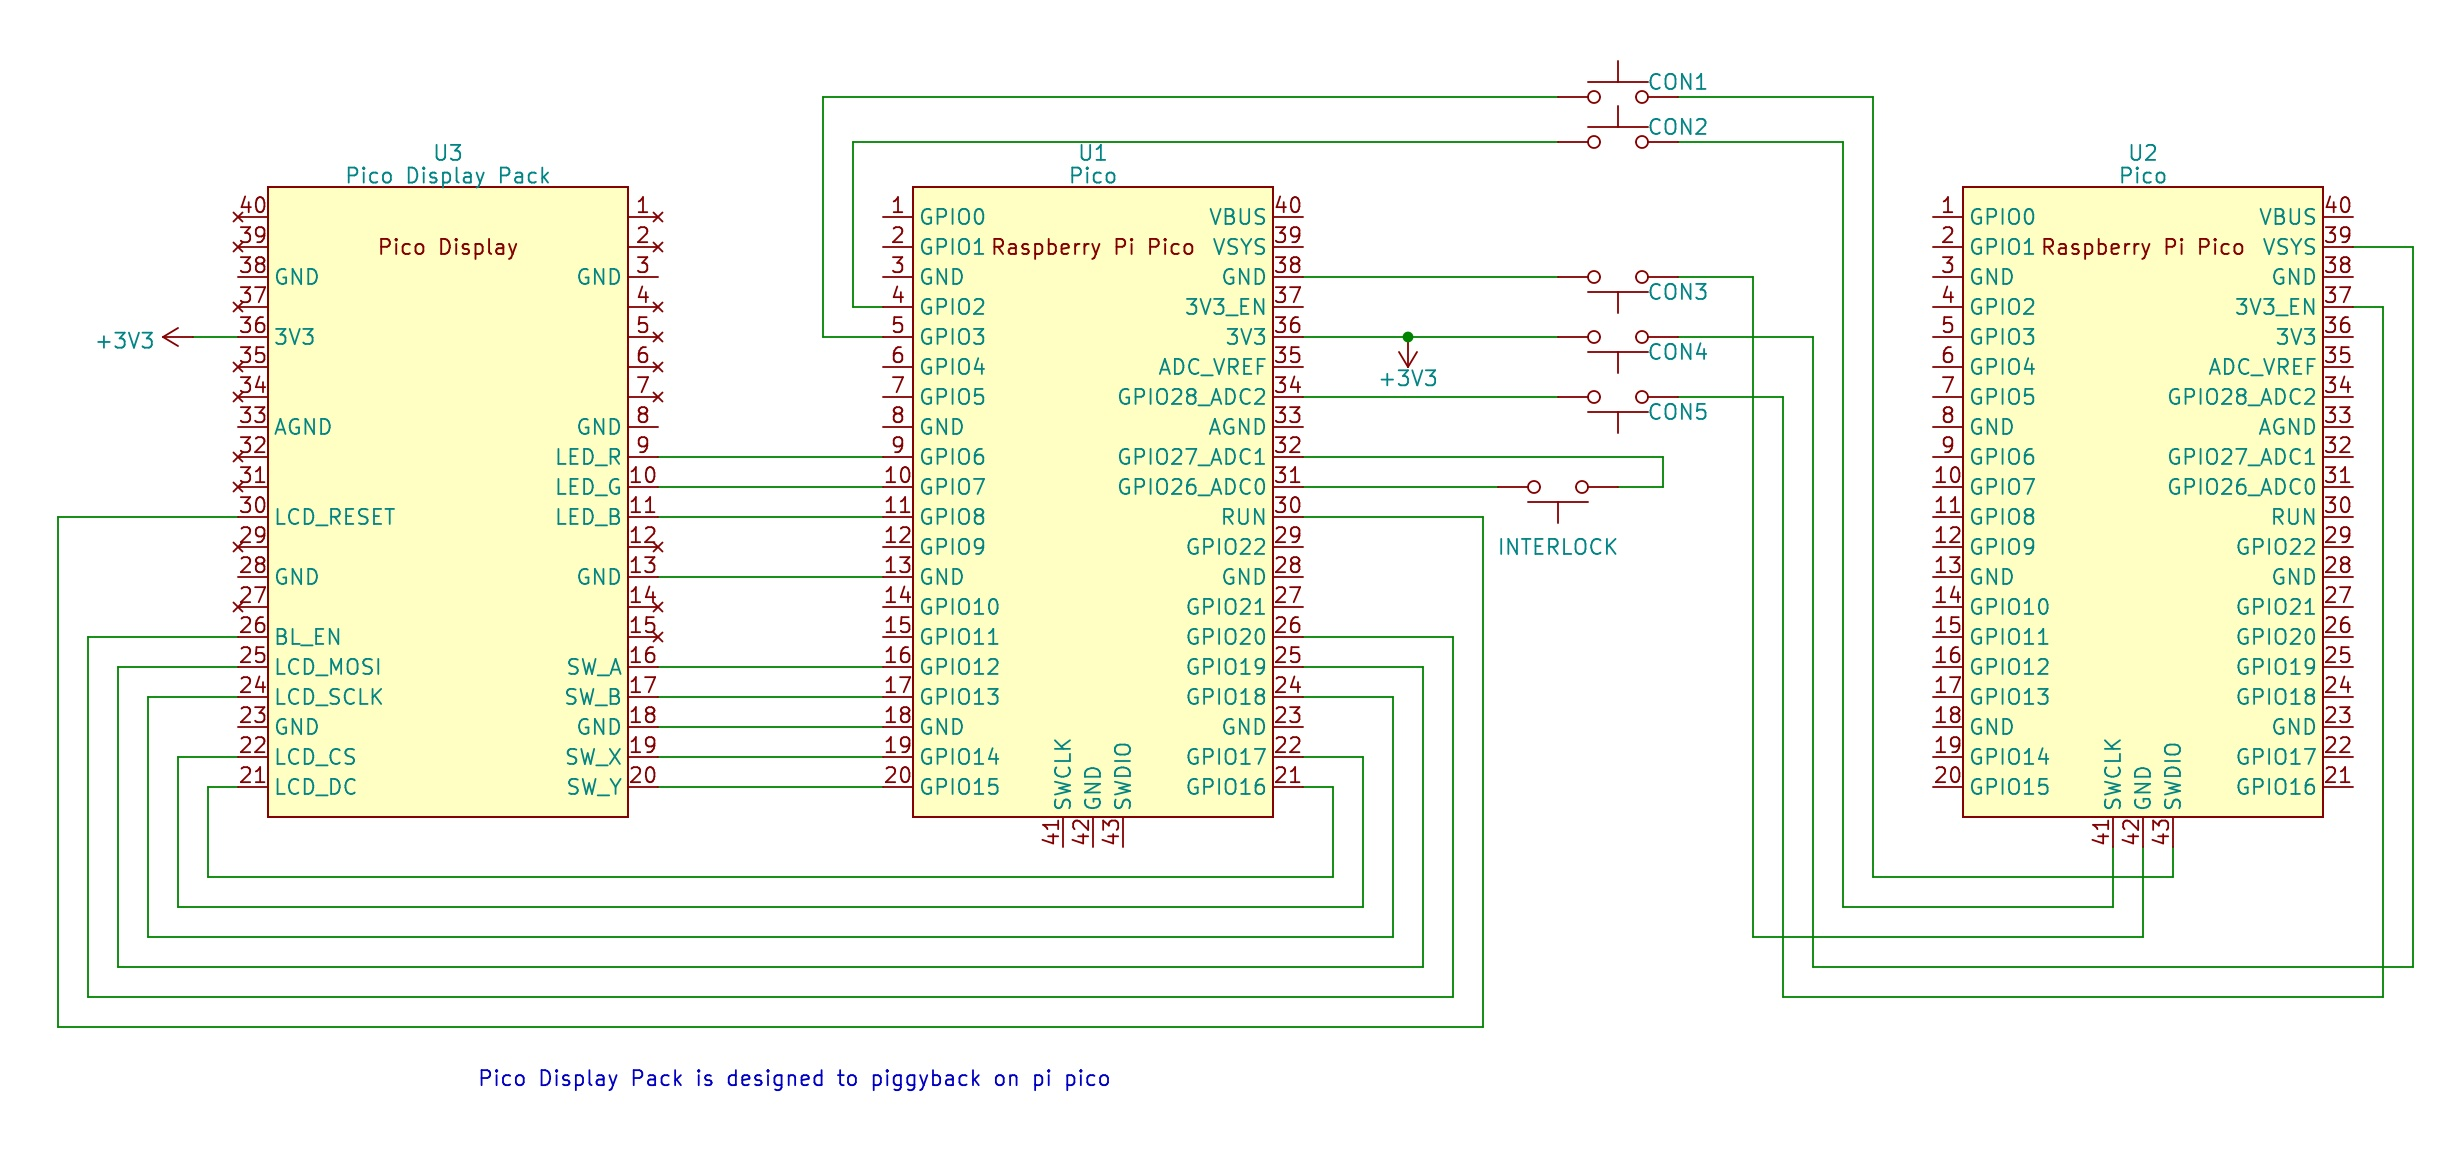
\includegraphics[width=\textwidth]{POC wiring schematic}}
	\caption{Wiring diagram for bench test hardware setup}
	\label{fig:FullPOCwiringDiagram}
\end{figure}
\clearpage
\section{Software bootstrap}
InInitial step was to establish \gls{swd} setup as lowest level critical component, this took longer than anticipated after initial response reading DPIDR register succeeded to verify an \gls{arm} debug unit was responding, but further attempted operations such as memory read failed. Reason for failure transpired to a lack of accounting multiple debug units\cite{raspberrypiltdRaspberryPiPico} with many references to \gls{swd} implementation omitting the step of device selection from the setup sequence owing to most \gls{arm} \gls{mcu}'s only having one core this being an unnecessary step.

Once handshake was established the most critical functions of memory write and read were implemented and verified to confirm successful control over \gls{swd}, 

From there a small \gls{ram} resident test program to blink the onboard \gls{led} was created as a test case binary to be write and executed from memory via \gls{swd} for a simple control verification, initially merely blinking \gls{led} to confirm code execution before building a shared memory structure for executing commands such as file recovery or flash programming/erasing.

This uses a \gls{magic} and runtime calculated CRC32 checksum for firmware data validation of transferred data during flashing process, and writing result codes back to memory that can be read by recovery device.

Programming sequence example to bootstrap running code on the target can be found in Appendix 1.

It was determined that 'bit banging' the \gls{swd} bus was sufficiently performant to not need a more complex implementation especially once the pico clock speed was increased from default 133MHz to a still stable and frequently used 250MHz.

Transferring the necessary 40kB helper image only takes 51ms to send over the bus which is inconsequential, and for  image upload operations the \gls{spi} flashing process is slower than the data upload  \gls{swd} speed, and most of the difference can be alleviated by using two data transfer locations to allow data upload whilst flashing is progressing in an interleaved write/transfer operation alternating locations.

This was measured to have approximately a 33\% speedup \autoref{table:flashspeed} in flashing versus using a single transfer location and waiting for write to complete before transferring new data.

\begin{table}[h]
	\centering
	\caption{Flashing speed with single and dual transfers}%IMPORTANT the caption must be before the tabular, so it will be on top of the table (there are other tricks to force it on top; but this one is straightforward).
	\vspace{-16.5pt}%time to time, spacing between caption and table can go too big...
	
	\begin{tabular}{|l|l|}
		\hline
		Flashing methodology & Time for MicroPython 1.19 Image transfer  \\ \hline
		Send and wait & 5562ms \\ \hline
		Dual interleave & 4154ms \\ \hline
	\end{tabular}
	\label{table:flashspeed}
\end{table}

To take control of target board, debug unit is first initialised to the rescue unit where a reset is performed, before switching over to regular debug unit and halting processor to ensure that the system is at a known state before uploading the  included sub helper binary image to handle flashing and recovery operations.

\clearpage
\section{File system implementation}

Due to the large amounts of repeated information and empty space within a UF2 format file direct storage into the pico's flash was impractical, especially with the effective requirement to store separate images for standard pico and W variations, which added together can reach a size bigger than the whole flash storage.

To enable maximum practical storage a more compact storage solution was implemented, consisting of three data areas for the UF2 image.

Laid out as follows: Data area, consisting of all the 256byte data packets from each UF2 block, An address area, indexing each of these data packets to their destination address and finally a header block where the filename, and other related metadata such as block count are stored. UF2 block /gls{crc} values were not stored and recalculated at runtime. Though a single checksum of all the data should still be added for verification before start of flashing.

Due to the requirement to store two images, there are two of these data structures kept, with the W one allocated the bulk of the storage to allow for the wireless module firmware and drivers taking up notably more storage than the regular pico as presented in table \ref{table:file_storage}:

\begin{table}[h]
	\centering
	\caption{Flash Storage layout}%IMPORTANT the caption must be before the tabular, so it will be on top of the table (there are other tricks to force it on top; but this one is straightforward).
	\vspace{-16.5pt}%time to time, spacing between caption and table can go too big...

		\begin{tabular}{|l|l|l|}
			\hline
			Address & Size  & Contents        \\ \hline
			0x000000 & 256kB & Program + Helper binary \\ \hline
			0x040000 & 4kB & UF2 Header 1      \\ \hline
			0x043000 & 12kB & UF2 Addresses 1 \\ \hline
			0x044000 & 600kB & UF2 Data 1 \\ \hline
			0x0D9000 & 4kB & UF2 Header 1 \\ \hline
			0x0DA000 & 20kB & UF2 Addresses 2      \\ \hline
			0x0DE000 & 1152kB & UF2 Data 2 \\ \hline
			0x1FFFFF & & End of flash. \\ \hline
		\end{tabular}
		\label{table:file_storage}
\end{table}

The \gls{usb} Virtual File System presented for UF2 image storage is based upon the TinyUF2 bootloader\cite{TinyUF2Bootloader2023}, which has been repurposed to capture file system uf2 transfer and store it to the internal UF2 storage.

To keep the files consistent even if power loss were to happen the file data is cleared at start of transaction, and header only written back once the full data is stored. Thus a power loss or other unexpected event mid transfer will leave the board with an empty file slot instead of inconsistent data.

One of the notable changes made to the TinyUF2 bootloader is to capture the file system information more fully, in order to read and store the full long file name of the UF2 image so that this can be presented to the user as an aid memoir on what firmware is loaded. This filename is also dynamically written to the virtual file system upon USB connection to present the data there also.

This required cacheing more of the \gls{fat} table than previously needed, due to long file names potentially requiring more than first cluster, especially with operating systems such as macOS that can also write other hidden helper files to the file system that need to be ignored.

Another modification over TinyUF2 loader is for the virtual image to present the currently stored image on the presented file system in recreated form when \gls{usb} loading is active including the current stored image size instead of presenting full flash image as originally designed, allowing end user to retrieve the image back off device as well as replace the stored image with an updated one.

\pagebreak
\section{Testing and UI}

For testing functionality, various likely scenarios were setup and verified to be repeatable.

First tests consisted of setting up recovery scenarios on MicroPython via Thonny\cite{ThonnyPythonIDE}, creating startup python scripts that both block the USB port or just run, and performing a recovery procedure to verify that the file is renamed successfully, or deleted, if a previous recovery result is still present.

Second tests verified that a populated file system could be wiped on an existing MicroPython install.

Third tests verified loading of different UF2 firmware files to the recovery platform, and then re imaging a target pico with the loaded firmware.

\clearpage
\subsection{USB Loading}
Figures \autoref{fig:picousbnodata} to \autoref{fig:usb_nodata_picow} show computer side of image loading in use, noting how the file system indicates which target device's firmware is being updated via use of dynamic text file name.

\begin{figure}[ht]
	\centering
	\AltText{File system shown on file system with no image loaded to device}{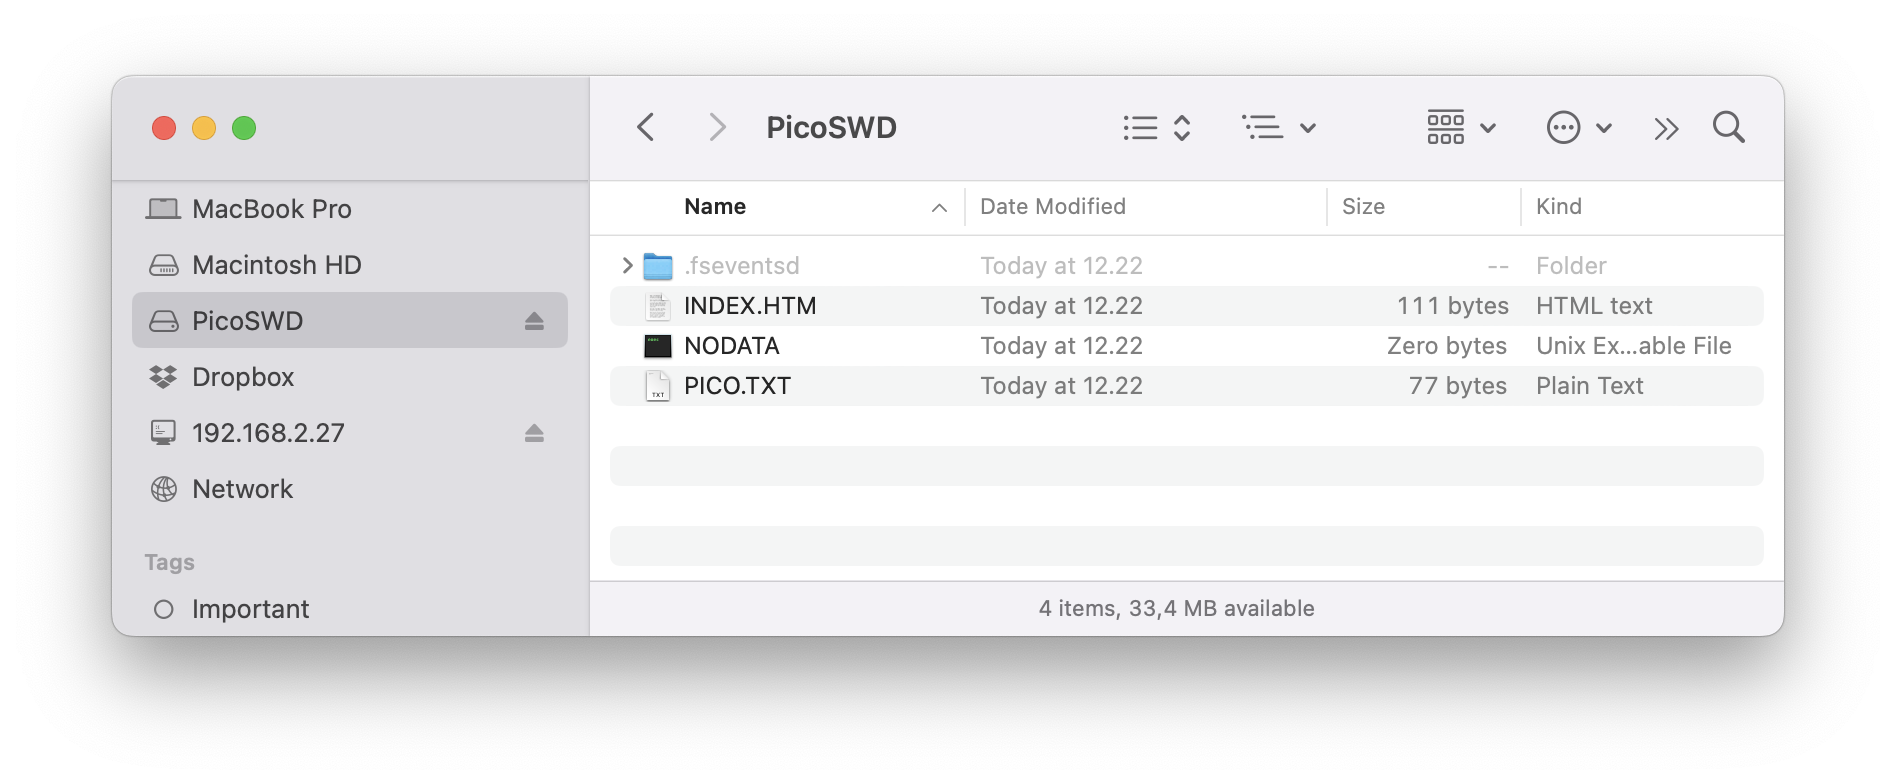
\includegraphics[width=\textwidth]{usb_nodata_pico}}
	\caption{Pico \gls{usb} image loading, no data}
	\label{fig:picousbnodata}
\end{figure}

\begin{figure}[ht]
	\centering
	\AltText{File system shown on file system with an image loaded to device}{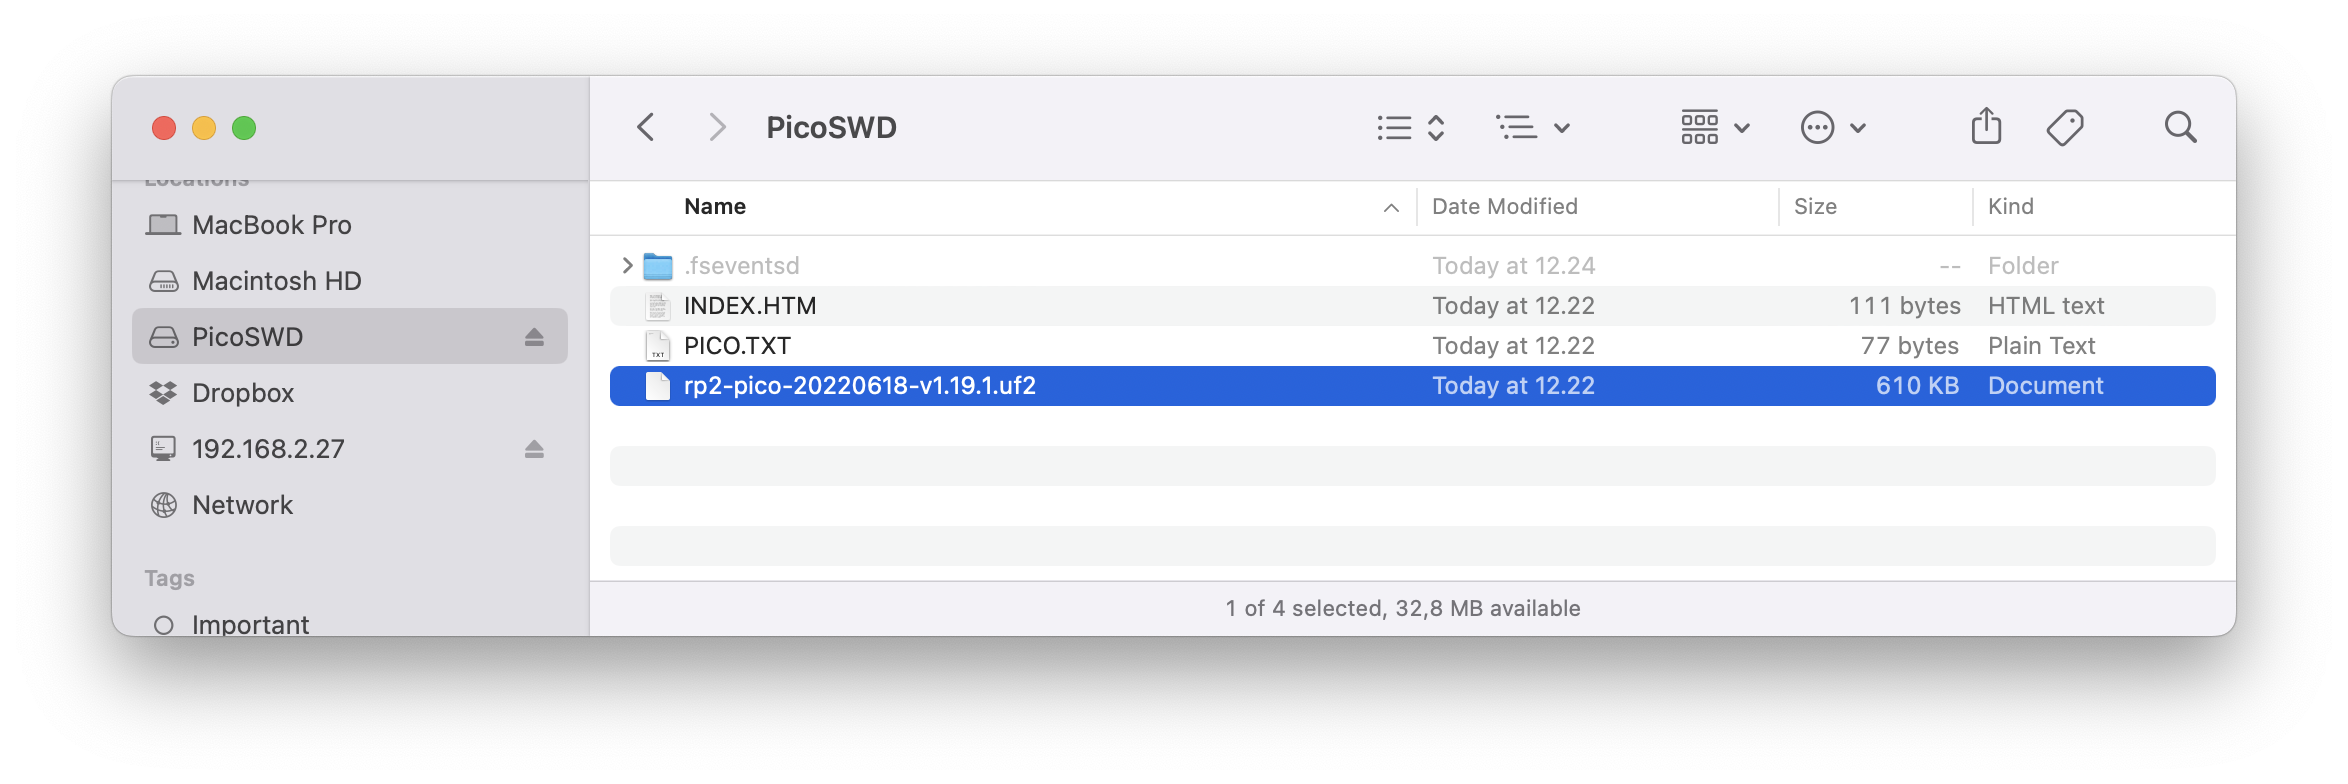
\includegraphics[width=\textwidth]{usb_data_pico}}
	\caption{Pico \gls{usb} image loading, MicroPython image loaded}
	\label{fig:picousbdata}
\end{figure}

\begin{figure}[ht]
	\centering
	\AltText{File system shown on file system with no image loaded to device}{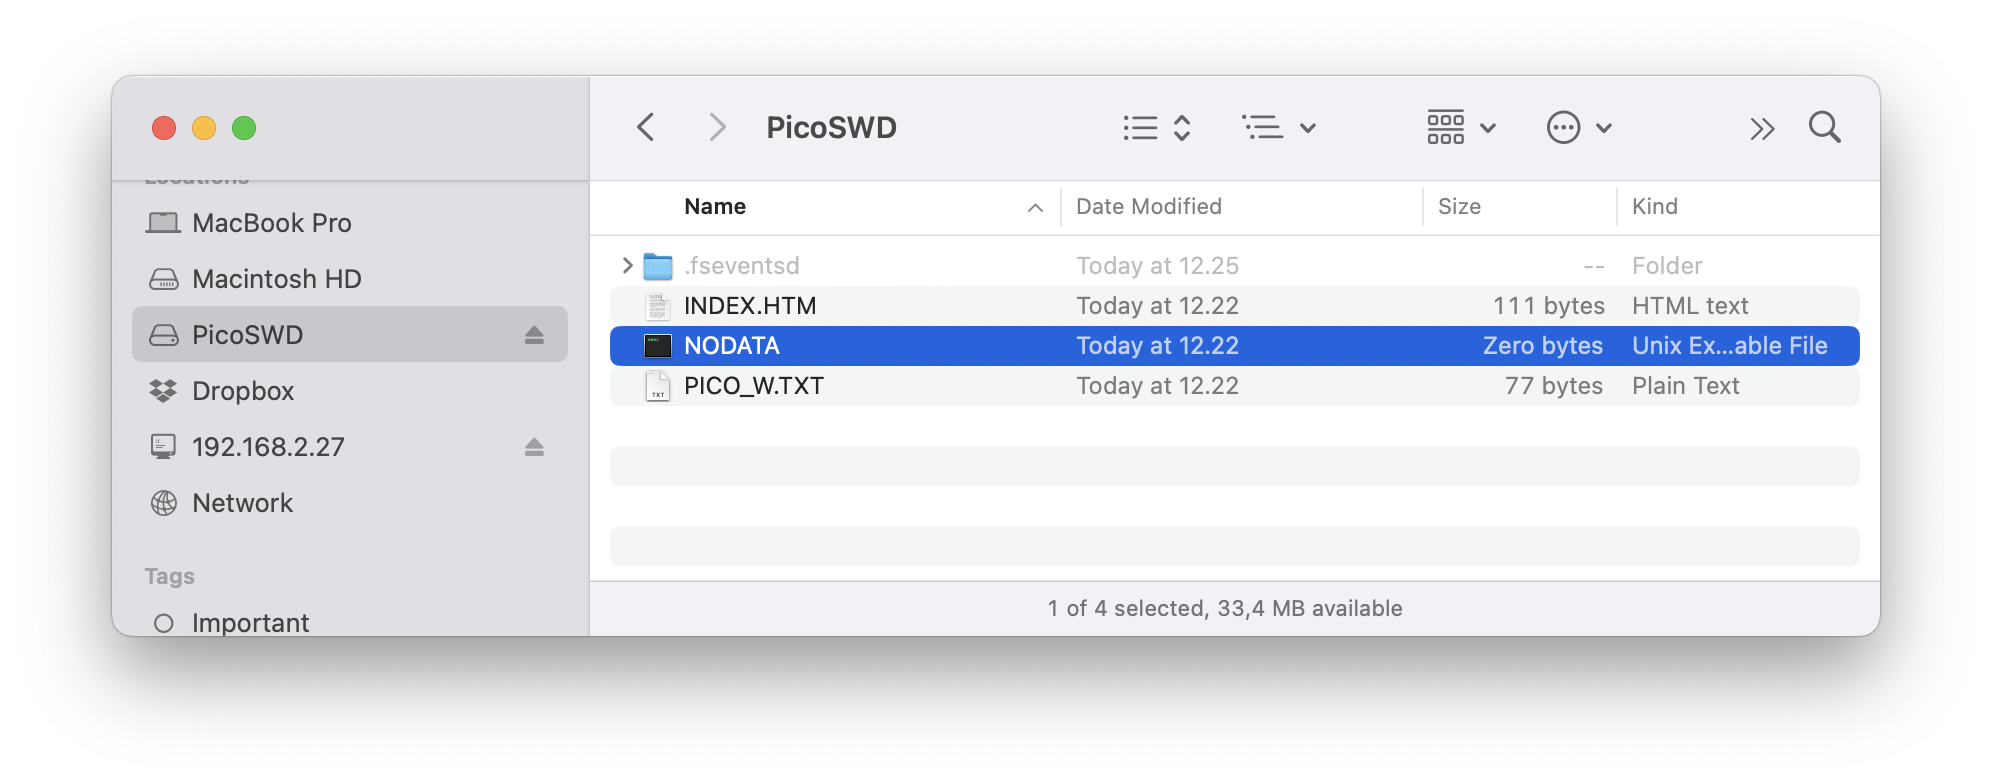
\includegraphics[width=\textwidth]{usb_nodata_picow}}
	\caption{Pico \gls{usb} image loading, no data}
	\label{fig:usb_nodata_picow}
\end{figure}

\clearpage
\subsection{Recovery Process}
Whilst figures \autoref{fig:disp_startup_empty} to \autoref{fig:disp_fs_recovered} demonstrate user interface on device at states of initial empty recovery and during \gls{usb} firmware loading, and further both file system recovery and re imaging a target device.

\begin{figure}[ht]
	\centering
	\AltText{Display startup no images stored}{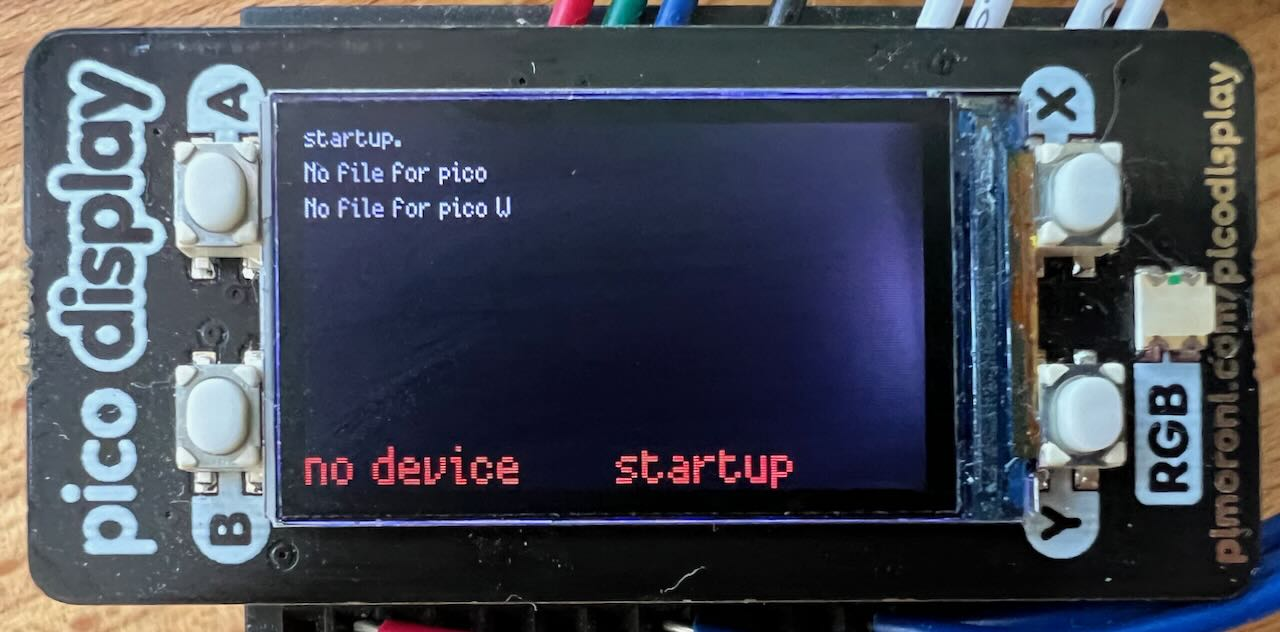
\includegraphics[width=.7\textwidth]{disp_startup_empty}}
	\caption{Display startup no images stored}
	\label{fig:disp_startup_empty}
\end{figure}

\begin{figure}[ht]
	\centering
	\AltText{Display startup Pico image stored}{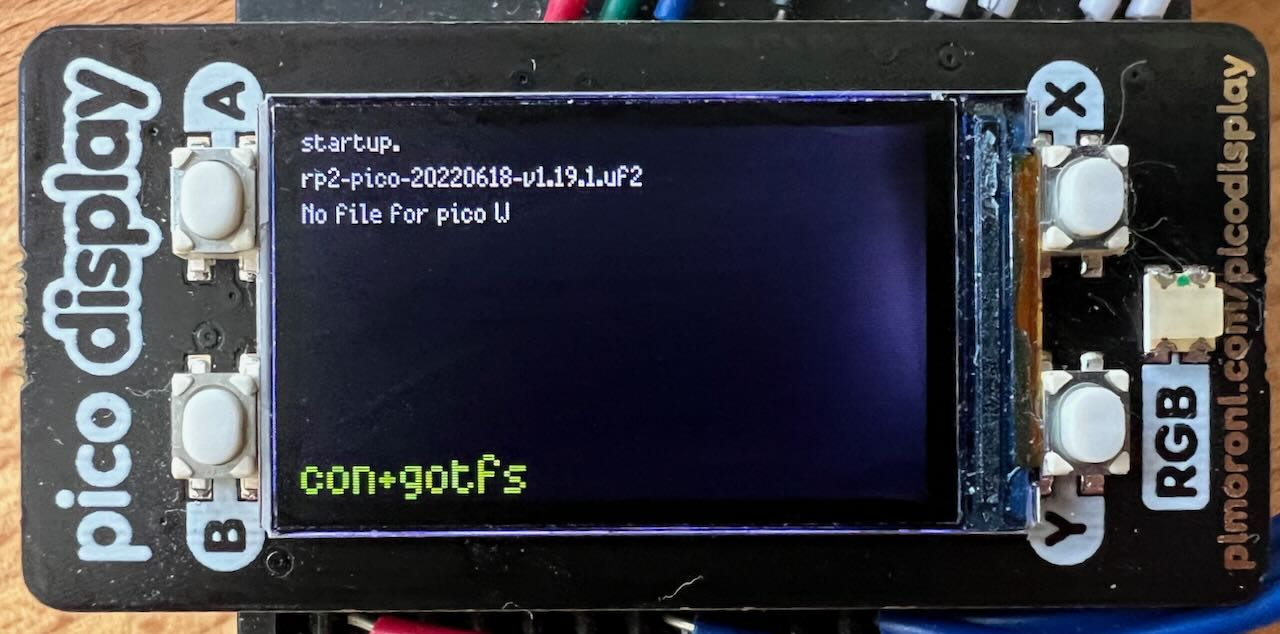
\includegraphics[width=.7\textwidth]{disp_startup_pico}}
	\caption{Display startup Pico image stored}
	\label{fig:disp_startup_pico}
\end{figure}

\begin{figure}[ht]
	\centering
	\AltText{Display showing recovery options menu}{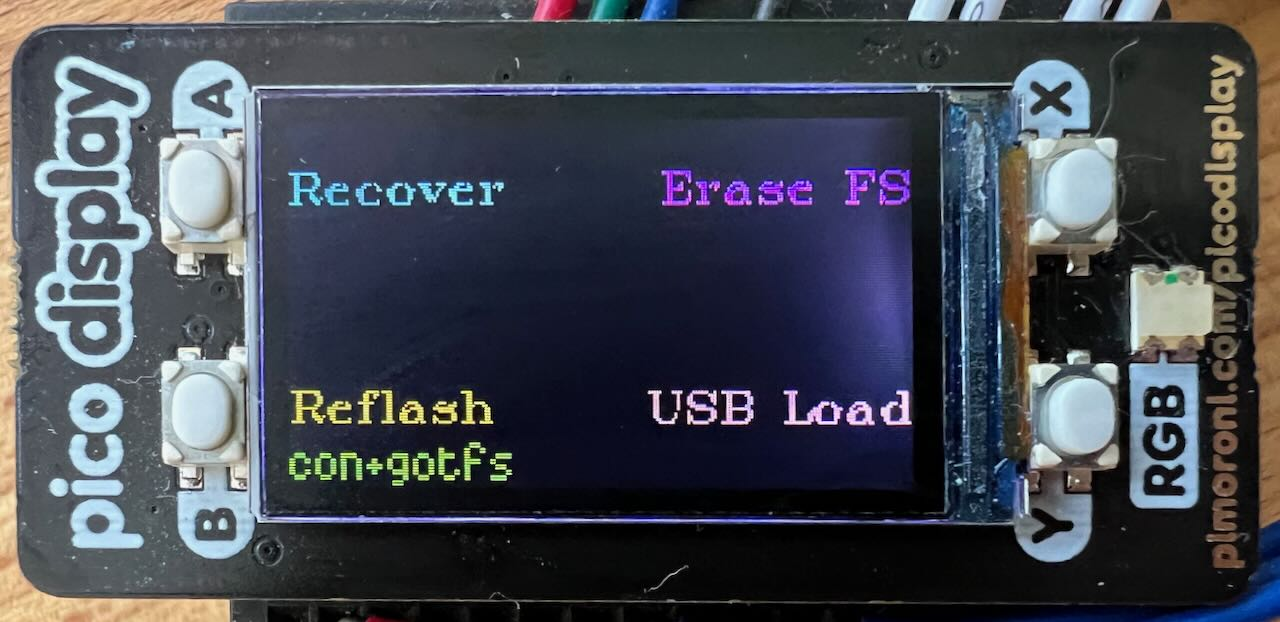
\includegraphics[width=.7\textwidth]{disp_menu}}
	\caption{Display showing recovery options menu}
	\label{fig:disp_menu}
\end{figure}

\begin{figure}[ht]
	\centering
	\AltText{Display showing USB image upload in progress at 58\%}{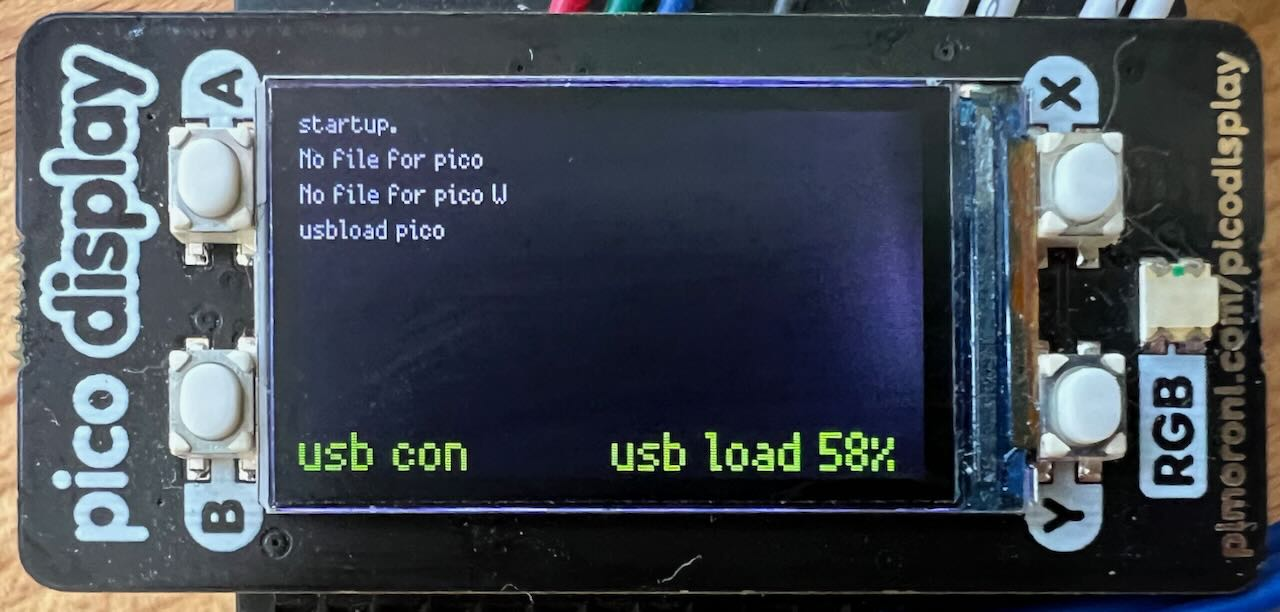
\includegraphics[width=.7\textwidth]{disp_usbload}}
	\caption{Display showing \gls{usb} image upload in progress}
	\label{fig:disp_usbload}
\end{figure}

\begin{figure}[ht]
	\centering
	\AltText{Display showing USB image having been uploaded}{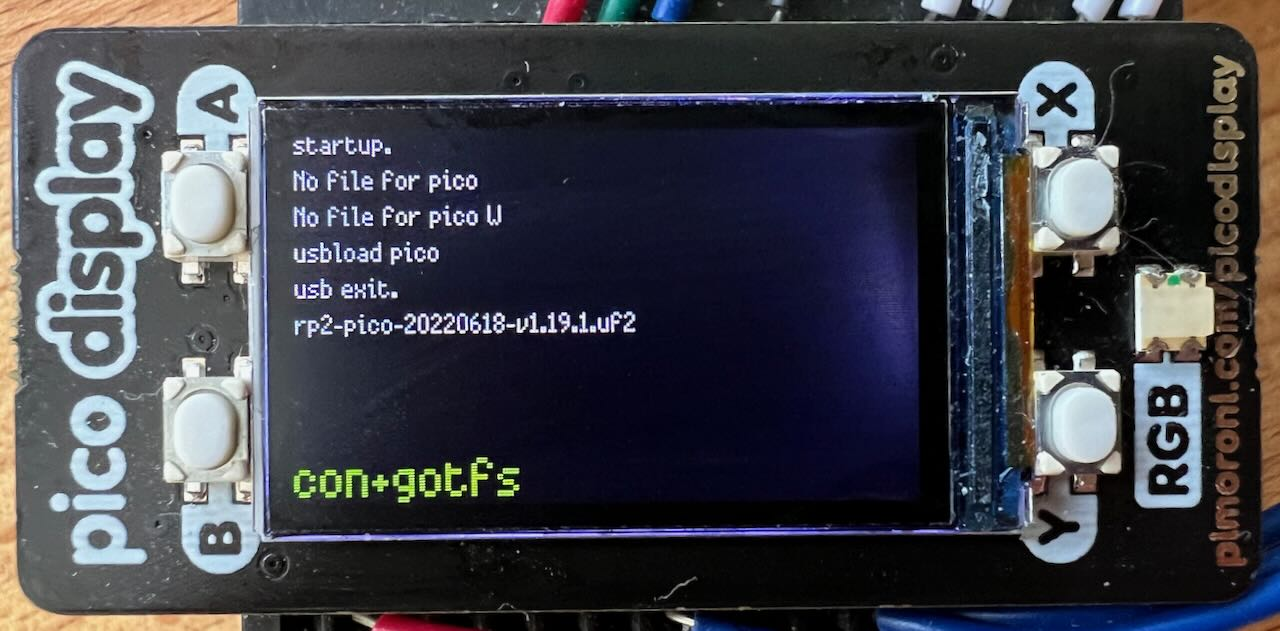
\includegraphics[width=.7\textwidth]{disp_usbloaded}}
	\caption{Display showing \gls{usb} image after successful upload}
	\label{fig:disp_usbloaded}
\end{figure}

\begin{figure}[ht]
	\centering
	\AltText{Display showing image flashing in progress}{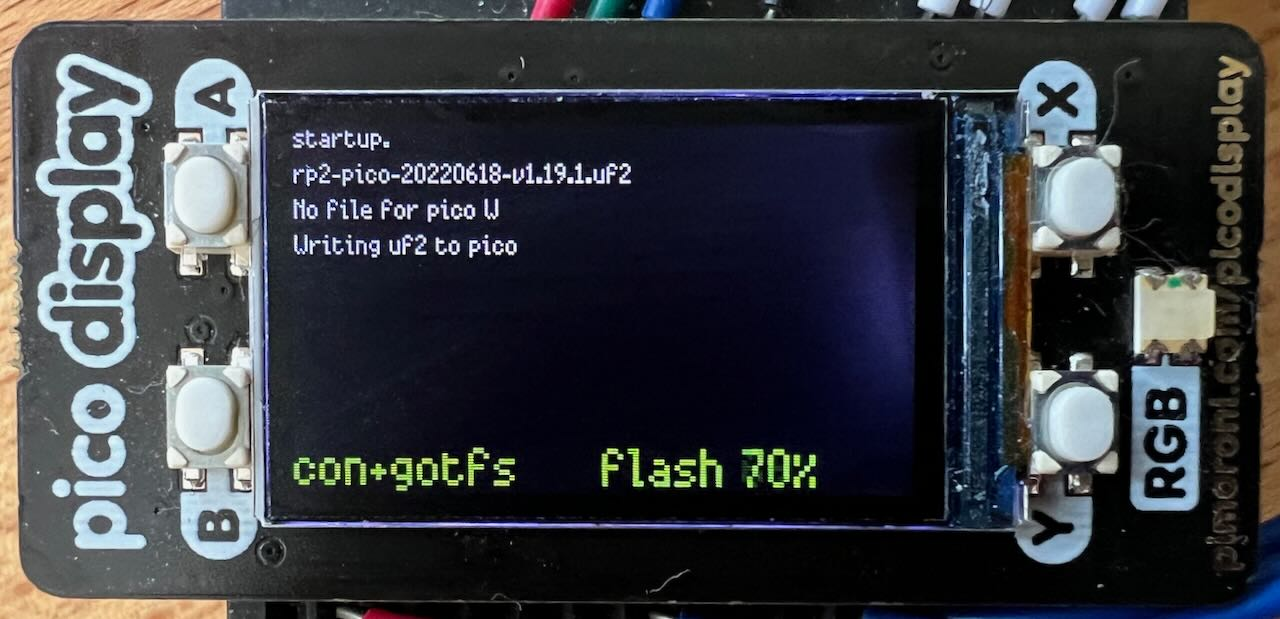
\includegraphics[width=.7\textwidth]{disp_flashwrite}}
	\caption{Display showing image flashing to target in progress}
	\label{fig:disp_flashwrite}
\end{figure}

\begin{figure}[ht]
	\centering
	\AltText{Display showing filesystem recovered}{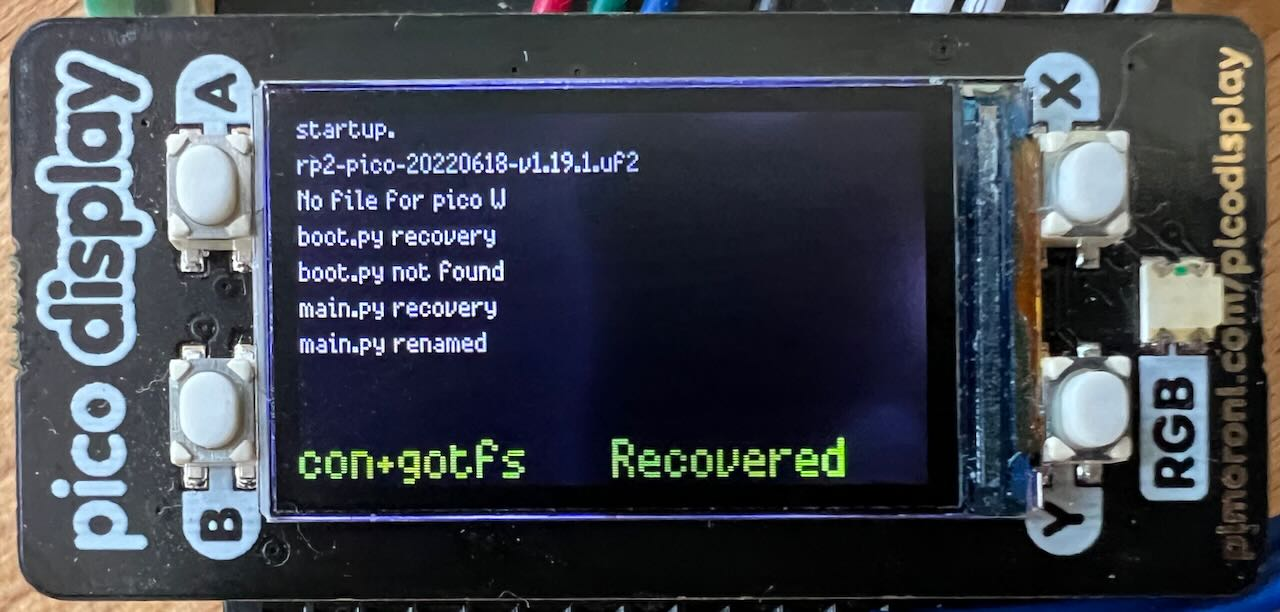
\includegraphics[width=.7\textwidth]{disp_fs_recovered}}
	\caption{Display showing successfully recovered filesystem}
	\label{fig:disp_fs_recovered}
\end{figure}



% Project Improvements remaining
\clearpage%if the chapter heading starts close to bottom of the page, force a line break and remove the vertical vspace
\vspace{21.5pt}
\chapter{Improvements and Challenges}

Whilst the software functionality attained the planned functionality there still remains hardware interface challenges that need to be solved to be a fully deployable solution.

Most notably there still needs to be a quick connection interface designed to allow a target board to be quickly attached to the recovery module. Multiple ways of making this connection have been considered, with the location of the debug points on the two board versions limiting the possibilities notably, especially with the Pico W where they are not located at a castellation making a fully side mounting clip an impossibility.  The most likely potential method to investigate being some form of mounting clip using pogo pins to make contact with at least the debugging connections, and potentially some kind of springclip or pogos for the power supply.

The enable pin could be left off design if power source is under direct control, being which could help simplify design further with only one point outside debug connector needed.

To aid with operation of a clip, the design features a pair of interlock circuit pins that are required to be closed together before power is supplied or enabled to the target board, this is intended to be some form of connection or switch that is activated after the other connections have been made to try and ensure all connections are closed before any function is performed.

 For simplicity of testing design, this control is currently implemented as controlling the power enable line of the voltage regulator on the target board, but should  be implemented as a MOSFET controlled direct power line or similar so that no power is supplied to the target board till full interlock is achieved, an example proposal of such a driver to control power supply and some simple extra protection resistors added to wiring in \autoref{fig:Wiringwithpowerdriver} using a transistor to drive a P channel MOSFET so that it would be controlled by a high GPIO signal and thus be in a known state at startup. This would entail some minor code changes to enable power once interlock is closed, but should result in a more robust circuit with lessened risk of misconnected pins allowing possible shorts or other unintended behaviour.

\begin{figure}[ht]
	\centering
	\AltText{Proposed extended interconnect design with power driver}{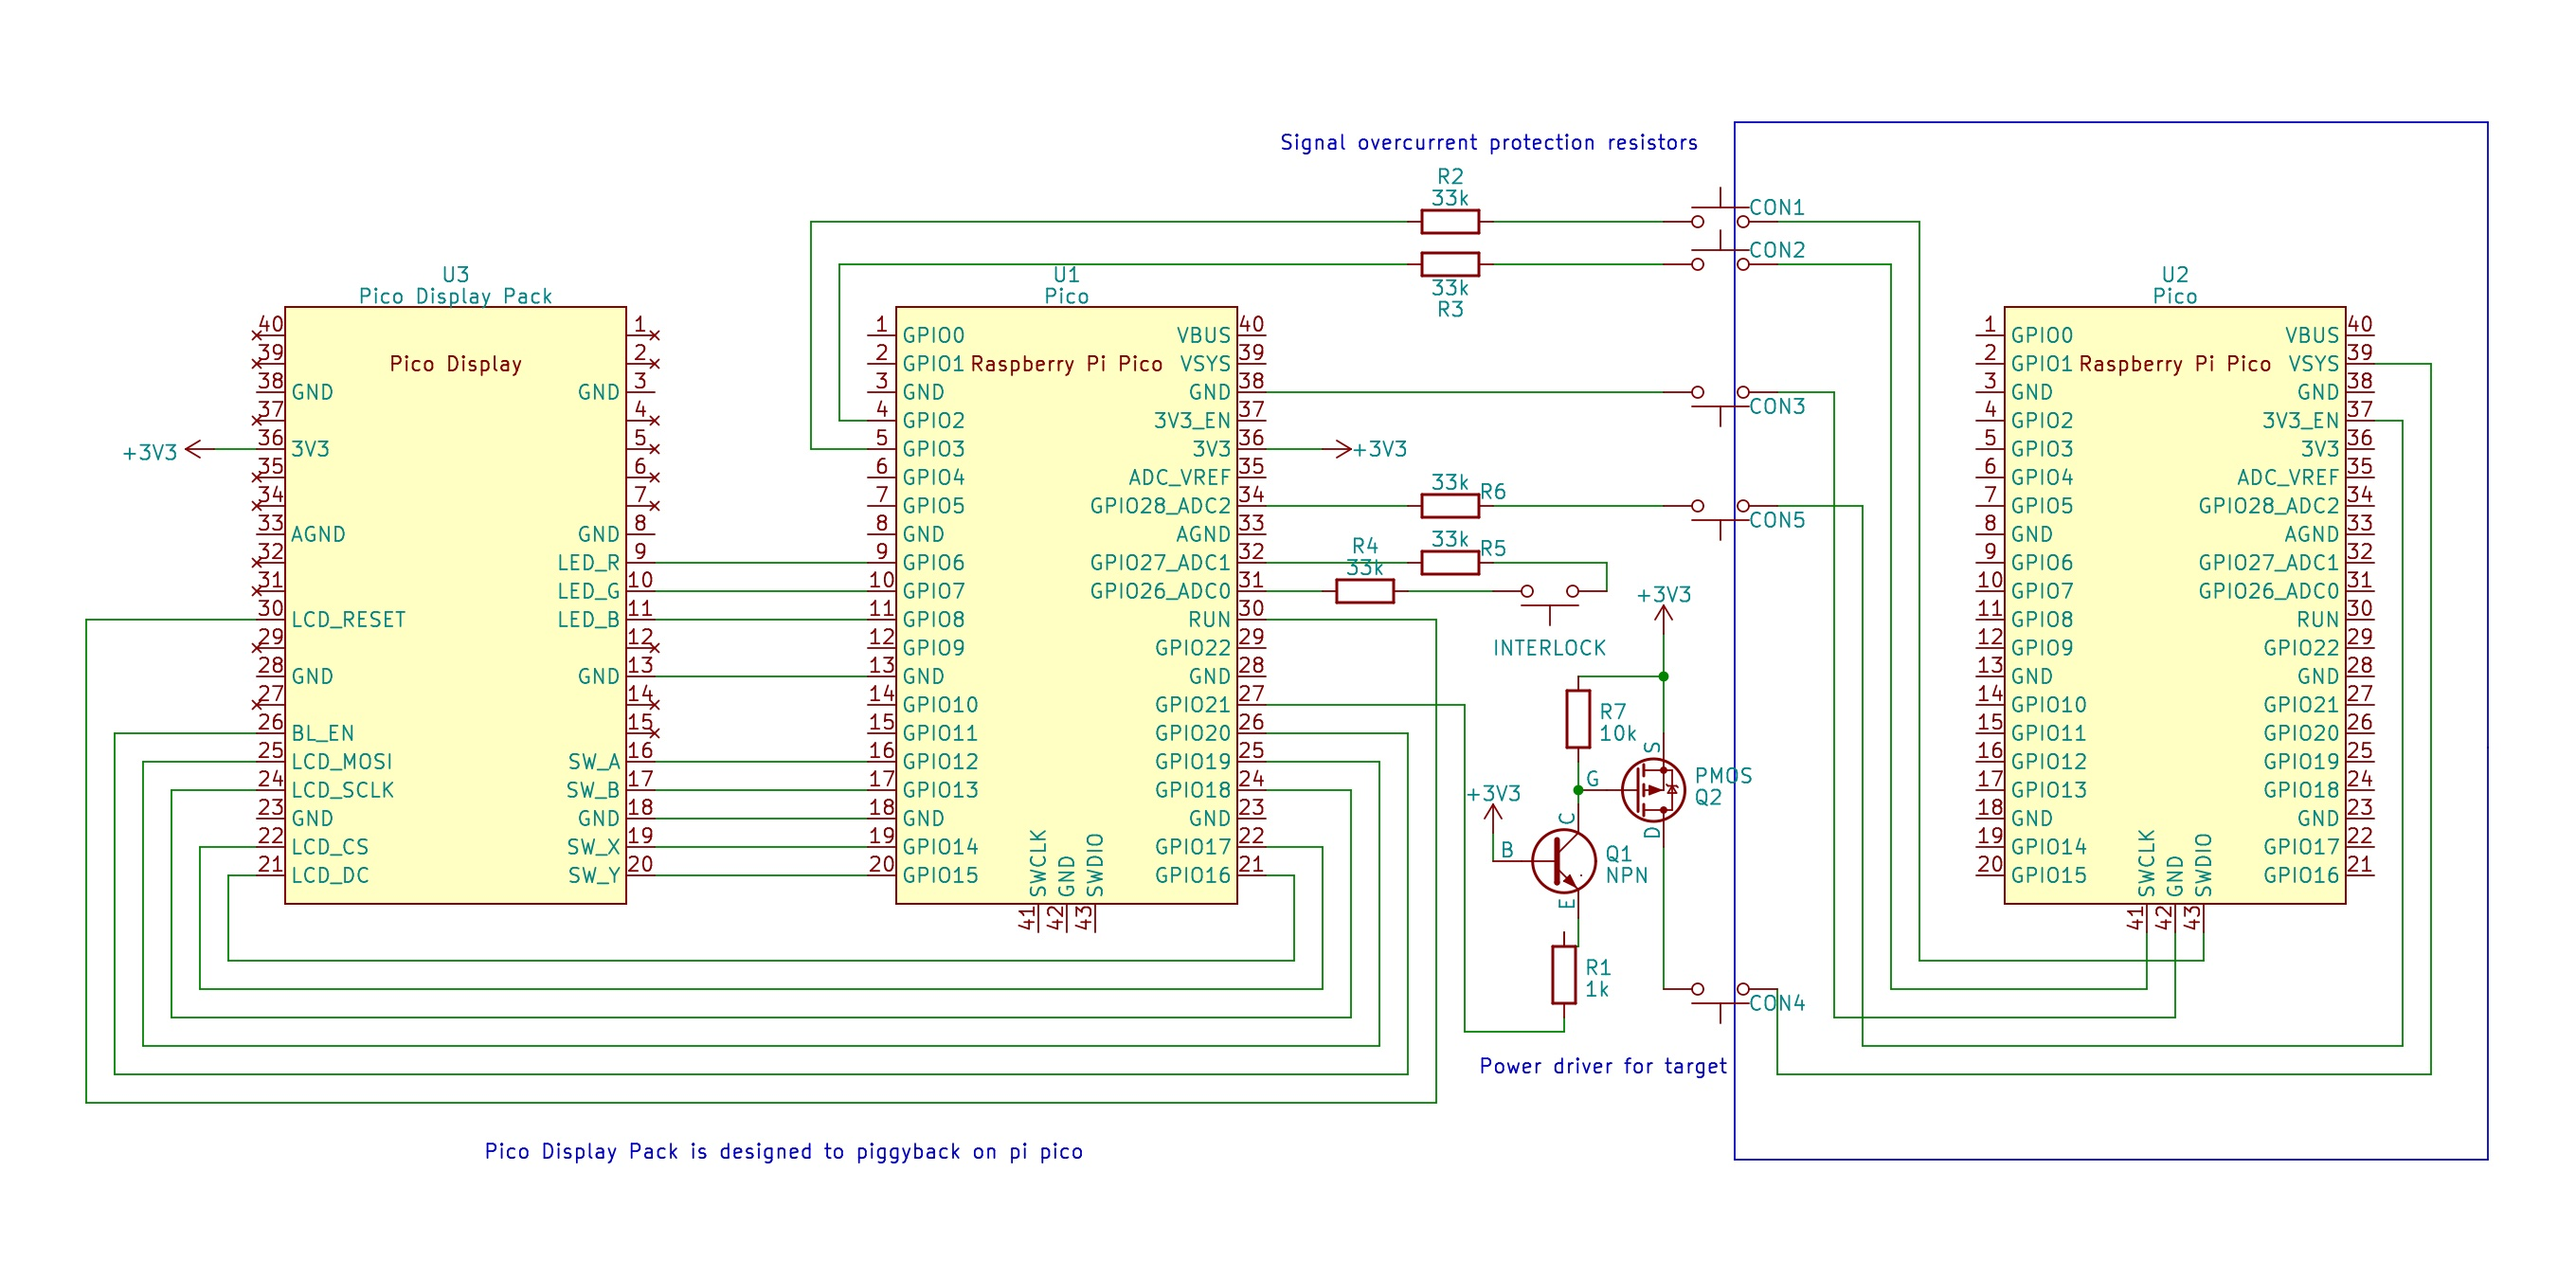
\includegraphics[width=\textwidth]{Schematic with power driver}}
	\caption{Wiring diagram including power driver}
	\label{fig:Wiringwithpowerdriver}
\end{figure}

Due to the test setup another potential is that the reliability of transmission over quick connect contactors has also not been established, which could potentially require more extensive error management. Though due to the relatively slow transmission speeds used in terms of possible SWD communication speeds, this is not anticipated to be a major concern, especially for simple recovery procedure where the helper application upload is verified before commencement and retried if necessary already and beyond this communication only involves writing small command packets to memory.

USB connectivity is also notably imperfect presently, especially regarding ejecting and disconnecting/reconnecting USB interface leading to occasional hanging states and need for restarting when connection is started or closed. Though due to updating images being a secondary less commonly performed function of the project, this was deemed to be sufficiently functional for current POC as connection is reliable once established.

Further minor improvements could still be made to file storage, file time and date are not presently stored but could be accomodated into header.
% Conclusion of project
\clearpage%if the chapter heading starts close to bottom of the page, force a line break and remove the vertical vspace
\vspace{21.5pt}
\chapter{Conclusion}

The project was largely a success, with good solutions to recovering and flashing the target board found and implemented.
%\input{chapters/methods.tex}
%\input{chapters/theory.tex}
%\input{chapters/solution.tex}
%\input{chapters/conclusion.tex}

% Sample content to demonstrate LaTeX command. You will likely delete this line and the
% next \input{sample/*} lines. You are also safe to delete the sample/ folder and its
% content once you refershed your LaTeX skills. Also check the appendix samples.
%%sample content to demonstrate LaTeX command.
\vspace{21.5pt}
\chapter{Demonstration Content}\label{demo:content}

This is a chapter to demonstrate some of the \gls{test} commands\cite{RaspberryPiPico} that you can use to format your text. If you are new to it, \gls{latex} follows the \gls{test} idea similar to \gls{test} where you concentrate on the content and structure and leave the formatting and styling to the computer. You will write your content in a plain text file\footnote{which can not get corrupted and can be put under version control} and indicate the structure with commands (similar to \gls{test} tags) then compile it to generate the pdf. Check some books or tutorials such as \LaTeX{} Wikibooks\footnote{\url{https://en.wikibooks.org/wiki/LaTeX}} and try with an online editor such as Overleaf\footnote{\url{https://www.overleaf.com/}} so you do not need to install the compiler on your computer first.

\section{Text, terms and abbreviations, figures, lists, etc.}

In \gls{latex}, the \mintinline{tex}{\textbf{bold}} command produces \textbf{bold}, \mintinline{tex}{\textit{italic}}  \textit{italic} and nesting \mintinline{tex}{\textbf{\textit{bolditalic}}} generates \textbf{\textit{bolditalic}}. If the goal is to semantically mark importance, then use \emph{emphasize} with \mintinline{tex}{\emph{emphasize}} command. That would take care of cases such as \mintinline{tex}{\textit{text in italic with \emph{important stuff} inside}} which will compile to \textit{text in italic with \emph{important stuff} inside}. Note that a paragraph is added by forcing a new line.

When one want to use an abbreviation or acronym like \gls{test} using the \mintinline{tex}{\gls{test}} command in \gls{latex}, the first time, it comes with it full version as can be seen in first paragraph of chapter \ref{demo:content} and for all next usages in its short form. Of course, when needed, the full version is available using e.g. the \mintinline{tex}{\acrlong{someID}} command. The defined terms like \gls{test} use the same \mintinline{tex}{\gls{test}} \gls{test} command. The Capitalized can be obtained with \mintinline{tex}{\Gls{id}}.

In this template, the abbreviations are defined in the \texttt{chapters/0abbr.tex} file with the \mintinline{tex}{\newacronym{id}{SHORT}{Long Form}} command. There can be many abbreviations and terms defined there, only the ones that are used in the text will be printed in the list of abbreviations (after table of content). And of course, it is the job of the compiler to sort them alphabetically. Should be avoided; but to have all the abbreviations and terms, even the non-used ones, use the \mintinline{tex}{\glsaddall} command before printing the list of abbreviations.

\begin{itemize}
  \item Check the thesis guide about the orphan list item (\mintinline{tex}{\item}): if only first item in the page, force a new page \mintinline{tex}{\clearpage} before \mintinline{tex}{\begin{itemize}}.
  \item When the list items are not sentences, they begin with a lowercase letter, and the last list item ends in a period.
  \item When the list items are sentences, they begin with a capitalized letter, and the list items end in a period. If item of the list contains a long text that spans multiple lines, the left edge aligns automatically.
\end{itemize}

And let also try the figure (see figure \ref{fig:latex-cover}) and internal reference (with \mintinline{tex}{\label{lbl:id}} and \mintinline{tex}{\ref{lbl:id}}). Alternative text is obtained with custom made \mintinline{tex}{\AltText{text}} command (using pdfcomment and accsupp packages). The reference can be done to any label, for example why not to appendix \ref{appx:first} or to appendix \ref{appx:second}? To note, \gls{latex} will place the figure to the best place (except with forcing). Let them float till the final of final edit\ldots ~then force them to not break a paragraph.%hugly hack... I'm sorry

\begin{figure}[ht]
  \centering
  \AltText{meaningful alternative description (e.g. LaTeX, from typeseting to genrated pdf)}{\includegraphics[width=7.1cm]{LaTeX_cover}}
  \caption{\gls{test} cover image (Copied from \citeauthor{wikibooks:latex} (\citedate{wikibooks:latex}) \cite{wikibooks:latex}).}
  \label{fig:latex-cover}
\end{figure}

According to the thesis guide, there must be a paragraph of text between figures/tables/listings and a chapter/(sub)section. And a paragraph is many sentences long like at least two.

\section{Bibliography references and citations}

Here is an example how to cite a bibliography entry \cite{kopka:guide} using the \\\mintinline{tex}{\cite{kopka:guide}} \gls{latex} command \cite[section 4.1]{tobias:book}. You might also like \mintinline{tex}{\citeauthor{some:id}} and \mintinline{tex}{\citedate{some:id}} ~as demonstrated in figure \ref{fig:latex-cover} caption and others like \mintinline{tex}{\citetitle{some:id}}, \mintinline{tex}{\citeurl{some:id}}, etc. To get very precise references, like chapter, section, pages number or range of a book, timing in video,\ldots that get indicated in square brackets in the command like \mintinline{tex}{\cite[04:01]{youtube:biblatex}} \cite[04:01]{youtube:biblatex}. Check the thesis guide, if the reference is only for the current sentence, the \mintinline{tex}{\cite{}} is placed before the dot, if the reference is for entire paragraph or group of sentences, then after the dot. If there is multiple sources for one sentence or paragraph, they have to be grouped together using the \mintinline{tex}{\cites[pp. 3, 5, 9--13]{some:id}[chap 4]{other:id}{more:id}{etc:id}} command. \cites[pp. 216--220]{kopka:guide}[chapter Special Pages, sections 3--4]{wikibooks:latex}[section 4.1]{tobias:book}[04:01--04:19]{youtube:biblatex}

Like for abbreviations, the bibliography entries are stored in a separated \texttt{biblio.bib} file and only the \mintinline{tex}{\cite}d ones will be printed in the bibliography references. There are many entry types such as \mintinline{tex}{@book}, \mintinline{tex}{@article}, \mintinline{tex}{@online}, \mintinline{tex}{@video}, \mintinline{tex}{@thesis} and many more, e.g. see \cite[section 2.1]{ctan:biblatex}. In the worst case, there is the \mintinline{tex}{@misc} fallback entry type. \gls{test} and biber compilers will take care of the numbering and sorting of the cited entries. Some tools help in managing the entries such as OttoBib\footnote{\url{http://www.ottobib.com/}} that will generate book entry from \gls{test} or ZoteroBib\footnote{\url{https://zbib.org/}} that can also take \gls{test}, \gls{test}, etc. It is also possible to get the entry form the IEEE Xplore\footnote{\url{https://ieeexplore.ieee.org/}} or Google Scholar\footnote{\url{https://scholar.google.com/}} as shown in figure \ref{fig:bibtex}. Of course, even if using such tools can greatly help, manual check/edit might be required (e.g. missing author,\ldots).

\begin{figure}[ht]
  \centering
  \AltText{getting BibTeX entries from Google Scholar and IEEE Xplore}{\includegraphics[width=\textwidth]{bibtex_gscholar_ieeexplore}}
  \caption{BibTeX entries from Google Scholar (left) or IEEE Xplore (right)}
  \label{fig:bibtex}
\end{figure}

Let's also try a long quote from the \citetitle{un:udhr}
\begin{quote}
(1) Everyone has the right to education. Education shall be free, at least in the elementary and fundamental stages. Elementary education shall be compulsory. Technical and professional education shall be made generally available and higher education shall be equally accessible to all on the basis of merit.

(2) Education shall be directed to the full development of the human personality and to the strengthening of respect for human rights and fundamental freedoms. It shall promote understanding, tolerance and friendship among all nations, racial or religious groups, and shall further the activities of the United Nations for the maintenance of peace.

(3) Parents have a prior right to choose the kind of education that shall be given to their children. \cite[article 26]{un:udhr}
\end{quote}

%TODO example with cite interview/conversation (unpublished or misc)
%https://tex.stackexchange.com/questions/111363/exclude-fullcite-citation-from-bibliography
\textit{Quisque augue} est, \textbf{elementum ac porttitor} non, porttitor ac orci. Donec hendrerit, ligula ac luctus egestas, sem dolor pretium nunc, sed vehicula magna diam a massa. Donec hstis, arcu et tempor mattis, risus tortor ultrices metus, nec sodales sem dolor eu elit.

Nullam egestas enim at odio pellentesque bibendum.

\subsection{Subsection}
Donec et sapien ac leo condimentum vulputate id et tellus. Maecenas hendrerit malesuada interdum. Aenean dignissim sem faucibus elit congue faucibus id non risus. Morbi at dui non tortor pellentesque consequat non eget urna. Cras in sapien dui, a tincidunt velit.
\reaction{\label{eq:reaktio}$\underset{\text{+II}}{\ce{2Fe^2+}}$ + $\underset{\text{+I\;-I}}{\ce{H2O2}}$ + $\underset{\text{+I\;-II}}{\ce{2H3O^+}}$ <=> $\underset{\text{+III}}{\ce{2Fe^3+}}$ + $\underset{\text{+I\;-II}}{\ce{4H2O}}$}
Työn aluksi rauta(II)ionit hapetetaan rauta(III)ioneiksi väkevällä vetyperoksidilla, kuten reaktion~\ref{eq:reaktio} hapetusluvuista nähdään (rauta hapettuu, happi pelkistyy).
\reaction{Fe^3+( \emph{aq} ) + 3OH^-( \emph{aq} ) + $(x-1)$H2O( \emph{l} ) -> FeOOH $\cdot$ $x$(H2O)( \emph{s} )}
Rauta(III)ionit saostetaan emäksen (\ce{NH3}) avulla ja saadaan tuotteeksi kidevedellinen rauta(III)hydroksidi. Saatu saostuma pestään \ce{NH4NO3}:lla.
\reaction{FeOOH $\cdot$ $x$(H2O)( \emph{s} ) ->T[$\Delta$900-1000\celsius] Fe2O3( \emph{s} )}

\subsection{Subsection with \texorpdfstring{\Gls{test}}{Mathematics}}%gls inside chapter/section/... will generate hyperref warning (link inside link in table of content), to avoid that, use the \texorpdfstring
Donec et sapien ac leo condimentum vulputate id et tellus. Maecenas hendrerit malesuada interdum. Aenean dignissim sem faucibus elit congue faucibus id non risus. Morbi at dui non tortor pellentesque consequat non eget urna. Cras in sapien dui, a tincidunt velit. Tertiäärinen butyylikloridi reagoi veden kanssa oheisen reaktion mukaisesti:
\reaction{(CH3)3CCl + 2H2O -> (CH3)3COH+H3O+ +Cl-}
Kyseessä on ensimmäisen kertaluvun reaktio, joten reaktion nopeus on
\begin{align}
v=-\frac{\mathrm{d}[\tn{t-ButCl}]}{\mathrm{d}t}=\frac{\mathrm{d}[\tn{HCl}]}{\mathrm{d}t}=k[\tn{t-ButCl}]
\end{align}
Jos tarkastellaan lähtöaineen t-butyylikloridin häviämistä saadaan
\begin{align}
\frac{\mathrm{d}[\tn{t-ButCl}]}{[\tn{t-ButCl}]}&=-k\mathrm{d}t \\
\int \frac{\mathrm{d}[\tn{t-ButCl}]}{[\tn{t-ButCl}]}&=-k \int \mathrm{d}t \\
\ln \int_{[\tn{t-ButCl}]_0}^{[\tn{t-ButCl}]} [\tn{t-ButCl}]&=-k\int_0^t t \\
\ln \left( \frac{[\tn{t-ButCl}]}{[\tn{t-ButCl}]_0} \right)&=-kt
\end{align}
Ionivahvuus lasketaan kaavalla.
\begin{align}
I&=\frac{1}{2}\cdot\sum z_i^2c_i \\
z_i&= \tn{ionin varausluku} \nonumber \\
c_i&= \tn{ionin konsentraatio} \nonumber
\end{align}
Aktiivisuuskerroin $\gamma_\pm$ lasketaan kaavalla.
\begin{align}
\log \gamma_\pm &= -\left|z_+\cdot z_-\right|A\cdot I^{\frac{1}{2}} \\
A &= \tn{0,509 (lämpötilassa 25\celsius}) \nonumber \\
I &= \tn{ionivahvuus} \nonumber \\
z &= \tn{ionien varaus} \nonumber
\end{align}

\section{Section with Source Code}
Donec et sapien ac leo condimentum vulputate id et tellus. Maecenas hendrerit malesuada interdum. Aenean dignissim sem faucibus elit congue faucibus id non risus. Morbi at dui non tortor pellentesque consequat non eget urna. Cras in sapien dui, a tincidunt velit.

%For sharelatex users, use space instead of tab to avoid ^^I
\begin{code}
  \begin{minted}{php}
<?php
$username = $_POST["username"];
//maybe not?
if ($userName){
  ?>
  <h2>Hello <?= $username ?>!</h2>
  <p>your message got received.</p>
  <?php
}
?>
\end{minted}
\captionof{listing}{Descriptive Caption Text (e.g. this \gls{fat} code do blah)}
  \label{code:testphp}
\end{code}


%As see in listing \ref{code:testphp}, blah. It is also possible to have code inline, for example \mintinline{fat}{SELECT * FROM user WHERE age >= 18} that was \gls{fat}.
The lisings \ref{code:htmlfull} and \ref{code:htmlpart} show how to load code from an external source file. In the case of listing \ref{code:htmlpart} it only take few line out of the source code file.

\begin{code}
  \inputminted{html}{code/html5_sample.html}
  \captionof{listing}{Some \gls{fat} code}
  \label{code:htmlfull}
\end{code}
 Donec et sapien ac leo condimentum vulputate id et tellus. Maecenas hendrerit malesuada interdum. Aenean dignissim sem faucibus elit congue faucibus id non risus.

 \begin{code}
   \inputminted[firstline=3,lastline=6]{html}{code/html5_sample.html}
   \captionof{listing}{The \mintinline{html}{<head>} section of an \gls{fat} page}
  \label{code:htmlpart}
\end{code}


 Morbi at dui non tortor pellentesque consequat non eget urna. Cras in sapien dui, a tincidunt velit.


\section{Section with Table}
Donec et sapien ac leo condimentum vulputate id et tellus. Maecenas hendrerit malesuada interdum. Aenean dignissim sem faucibus elit congue faucibus id non risus. Morbi at dui non tortor pellentesque consequat non eget urna. Cras in sapien dui, a tincidunt velit.

\begin{table}[h]
  \centering
  \caption{Some data}%IMPORTANT the caption must be before the tabular, so it will be on top of the table (there are other tricks to force it on top; but this one is straightforward).
  \vspace{-16.5pt}%time to time, spacing between caption and table can go too big...
  \begin{tabular}{| l | >{\centering\arraybackslash}p{.5\textwidth} |}
    \hline
    Test 1 & test 1234 test \\
    \hline
    Some more data comes here & with more values and if the text is very long it will disappear out of the box unless you force the column size :( You can use e.g. \textbackslash raggedright or \textbackslash centering (as in this example) to avoid hyphenization of long words\ldots \\
    \hline
  \end{tabular}
  \label{table:some_data}
\end{table}

As presented in table \ref{table:some_data}: Donec et sapien ac leo condimentum vulputate id et tellus. Maecenas hendrerit malesuada interdum. Aenean dignissim sem faucibus elit congue faucibus id non risus. Morbi at dui non tortor pellentesque consequat non eget urna. Cras in sapien dui, a tincidunt velit.

\begin{table}[h]
  \centering
  \caption{Another table with tabularx}
  \begin{tabularx}{.95\textwidth}{| l | >{\centering\arraybackslash} X |}
    \hline
    Test 1 & test 1234 test \\
    \hline
    Some more data comes here & with more values and if the text is very long it will disappear out of the box unless you force the table size :( \\
    \hline
  \end{tabularx}
  \label{table:some_data2}
\end{table}

As presented in table \ref{table:some_data2}: Donec et sapien ac leo condimentum vulputate id et tellus. Maecenas hendrerit malesuada interdum. Aenean dignissim sem faucibus elit congue faucibus id non risus. Morbi at dui non tortor pellentesque consequat non eget urna. Cras in sapien dui, a tincidunt velit.

Donec et sapien ac leo condimentum vulputate id et tellus. Maecenas hendrerit malesuada interdum. Aenean dignissim sem faucibus elit congue faucibus id non risus. Morbi at dui non tortor pellentesque consequat non eget urna. Cras in sapien dui, a tincidunt velit.

\begin{table}[htbp]
  \centering
  \caption{Booktabs example}
  \vspace{-16.5pt}
    \begin{tabular}{rrrr}
    \toprule
    t (s) & [HCl] & [t-ButCl] & $\ln\frac{[t-ButCl]}{[t-ButCl]_0}$ \\
    \midrule
    0     & 4,02  & 160,88 & 0,00 \\
    10    & 63    & 101,9 & -0,46 \\
    20    & 115,2 & 49,7  & -1,17 \\
    30    & 141,3 & 23,6  & -1,92 \\
    40    & 157,9 & 7     & -3,13 \\
    50    & 161   & 3,9   & -3,72 \\
    60    & 164,3 & 0,6   & -5,59 \\
    70    & 163,5 & 1,4   & -4,74 \\
    80    & 163,8 & 1,1   & -4,99 \\
    90    & 164,1 & 0,8   & -5,30 \\
    100   & 164,3 & 0,6   & -5,59 \\
    \bottomrule
    \end{tabular}
  \label{tab:thisislabel}
\end{table}

As presented in table \ref{tab:thisislabel}: Donec et sapien ac leo condimentum vulputate id et tellus. Maecenas hendrerit malesuada interdum. Aenean dignissim sem faucibus elit congue faucibus id non risus. Morbi at dui non tortor pellentesque consequat non eget urna. Cras in sapien dui, a tincidunt velit.

%\input{sample/2lorem.tex}
%\input{sample/3graph.tex}

%----------------------------------------------------------------------------------------
%	BIBLIOGRAPHY REFERENCES
%----------------------------------------------------------------------------------------

\input{style/biblio.tex}

%----------------------------------------------------------------------------------------
%	APPENDICES
%----------------------------------------------------------------------------------------

\input{style/appendix.tex}
%force smaller vertical spacing in table of content
%!!! There can be some fun depending if the appendices have (sub)sections or not :D
% You will have to play with these numbers and eventually add the \vspace line  before
% some \chapter and force another number.
% To add more fun, time to time the table of content get wrong after a build :(
\addtocontents{toc}{\vspace{11pt}}
\pretocmd{\chapter}{\addtocontents{toc}{\protect\vspace{-24pt}}}{}{}

\liite{1}% This is a hack to have right page numbering for each appendix. Make sure to
% use a unique number for each appendix.
% Appendix
% And demonstrate text references and bibliography references in appendix

\chapter{Running code over SWD}\label{appx:first}

\begin{code}
	\begin{minted}{c}
bool probe_sendhelper( void )
{
	// send the recovery program
	probe_write_dp(swdpreg_wo_SELECT, 0);
	probe_write_dp(swdpreg_rw_CSR,
	( 1 << ORUNDETECT )
	//| ( 1 << READOK )
	| ( 1 << CDBGPWRUPREQ )
	| ( 1 << CSYSPWRUPREQ ) );
	
	uint32_t reg = 0;
	probe_read_dp(swdpreg_rw_CSR, &reg);
	if ( reg ==       ( 1 << ORUNDETECT )
	| ( 1 << CDBGPWRUPREQ )
	| ( 1 << CDBGPWRUPACK )
	| ( 1 << CSYSPWRUPREQ ) 
	| ( 1 << CSYSPWRUPACK ) )
	{
		printf("CSR ok\n");
	}
	
	if ( ! probe_write_ap(ahbap_rw_CSW, 
	( APSIZE32BIT << MEMAPSIZE )
	| ( ADDRINCSINGLEEN << ADDRINC )  
	| ( 1 << APDEVICEEN )
	| ( 0b0100010 << APPROT )
	| ( 1 << DBGSWENABLE) ) )
	{
		printf("Setup error 1\n"); 
	}
	
	if ( ! probe_write_ap(ahbap_rw_TAR, DHCSR) ) // Debug Halting Control and Status Register
	{
		printf("Setup error 2\n");
	}
	if (! probe_write_ap(ahbap_rw_DRW, 0xA05F0003) ) // set debug enable and halt CPU.
	{
		printf("Setup error 3\n");
	}
	
	printf("Send helper %dB\n", sizeof _Users_visa_Code_pico_picorecover_wipe_build_wipe_bin);
	uint32_t start = time_us_32();
	probe_write_memory(0x20000000, _Users_visa_Code_pico_picorecover_wipe_build_wipe_bin, sizeof _Users_visa_Code_pico_picorecover_wipe_build_wipe_bin);
	printf("Send took %dms, Checking helper %dB\n", (time_us_32() - start)/1000, sizeof _Users_visa_Code_pico_picorecover_wipe_build_wipe_bin);
	start = time_us_32();
	
	printf("Verify data:\n"); 
	if ( !probe_verify_memory(0x20000000, _Users_visa_Code_pico_picorecover_wipe_build_wipe_bin, sizeof _Users_visa_Code_pico_picorecover_wipe_build_wipe_bin) )
	{
		printf("Verify failed, Bad data send\n"); 
	}
	
	printf("Read took %dms\n", (time_us_32() - start)/1000);
	
	bool waiting = true;
	uint32_t magiccheck = 0;
	
	uint8_t empty[12] = {0};
	if ( ! probe_write_memory(0x20038000, empty, 12) )
	{
		printf("Clear error\n");
	}
	magiccheck = 0;
	if ( ! probe_read_memory( 0x20038000, (uint8_t*)&magiccheck, sizeof magiccheck) || magiccheck != 0)
	{
		printf("Initial magic error\n");
	}
	
	// start execution.
	probe_write_ap(ahbap_rw_TAR, DCRDR); // Debug Core Register Data Register
	probe_write_ap(ahbap_rw_DRW, 0x20000000);
	probe_write_ap(ahbap_rw_TAR, DCRSR); // Debug Core Register Selector Register
	probe_write_ap(ahbap_rw_DRW, 0x0001000F);
	// DebugReturnAddress << REGSEL Sets execution address on leaving debug state.
	//    1 << DCRSRWRITE
	// bit 16 -- write access
	// 0b1 0000 0000 0000 1111
	probe_write_ap(ahbap_rw_TAR, DHCSR); // DHCSR	RW	0x00000000	Debug Halting Control and Status Register
	probe_write_ap(ahbap_rw_DRW, 0xA05F0001); // remove halt bit.
	
	uint32_t magic = 0xDEADBEEF;
	
	printf("Waiting magic to confirm execution started\n");
	
	sleep_ms(50); // seems to sometimes need a small delay after execution starts to get a non error read?
	
	start = time_us_32();
	do
	{
		magiccheck = 0;
		if ( !probe_read_memory( 0x20038000, (uint8_t*)&magiccheck, sizeof magiccheck) )
		{
			printf("magic read error\n");
			//return false;
		}
		if ( magiccheck == magic )
		{
			printf("Got confirmation: %08x\n", magiccheck);
			return true;
		}
		sleep_ms(100);
	} while ( time_us_32() - start < 3000*1000 );
	
	printf("Timeout waiting for magic.\n");
	
	return false;
}
	\end{minted}
	\captionof{listing}{C Function to upload and execute code on target RP2040}
	\label{code:probe_sendhelper}
\end{code}

The listed code demonstrated the steps needed to send and start arbitrary code executing on the target RP2040 platform,

consisting of halting CPU, uploading and verifying the binary data to memory then proceeding to setup the cpu to restart execution from the start of the uploaded code at base RAM address.

%\section{Appendix Section}

%And you can cite \cite{tobias:book} stuff, it will go into the main bibliography.% Sample content to demonstrate appendix in LaTeX. You
% are safe to delete this lines (and the next samples) once you refreshed your LaTeX
% skills (and safe to delete the sample folder and all its file too).

\addtocontents{toc}{\vspace{11pt}}%fix vertical space for Table of Content
\liite{2}
% Appendix
% Just to have more appendices and more content

\chapter{Second Appendix}\label{appx:second}



%\addtocontents{toc}{\vspace{11pt}}
%\liite{3}
%\input{sample/X_R_example.tex}
%sample content to demonstrate LaTeX command.
\vspace{21.5pt}
\chapter{Demonstration Content}\label{demo:content}

This is a chapter to demonstrate some of the \gls{test} commands\cite{RaspberryPiPico} that you can use to format your text. If you are new to it, \gls{latex} follows the \gls{test} idea similar to \gls{test} where you concentrate on the content and structure and leave the formatting and styling to the computer. You will write your content in a plain text file\footnote{which can not get corrupted and can be put under version control} and indicate the structure with commands (similar to \gls{test} tags) then compile it to generate the pdf. Check some books or tutorials such as \LaTeX{} Wikibooks\footnote{\url{https://en.wikibooks.org/wiki/LaTeX}} and try with an online editor such as Overleaf\footnote{\url{https://www.overleaf.com/}} so you do not need to install the compiler on your computer first.

\section{Text, terms and abbreviations, figures, lists, etc.}

In \gls{latex}, the \mintinline{tex}{\textbf{bold}} command produces \textbf{bold}, \mintinline{tex}{\textit{italic}}  \textit{italic} and nesting \mintinline{tex}{\textbf{\textit{bolditalic}}} generates \textbf{\textit{bolditalic}}. If the goal is to semantically mark importance, then use \emph{emphasize} with \mintinline{tex}{\emph{emphasize}} command. That would take care of cases such as \mintinline{tex}{\textit{text in italic with \emph{important stuff} inside}} which will compile to \textit{text in italic with \emph{important stuff} inside}. Note that a paragraph is added by forcing a new line.

When one want to use an abbreviation or acronym like \gls{test} using the \mintinline{tex}{\gls{test}} command in \gls{latex}, the first time, it comes with it full version as can be seen in first paragraph of chapter \ref{demo:content} and for all next usages in its short form. Of course, when needed, the full version is available using e.g. the \mintinline{tex}{\acrlong{someID}} command. The defined terms like \gls{test} use the same \mintinline{tex}{\gls{test}} \gls{test} command. The Capitalized can be obtained with \mintinline{tex}{\Gls{id}}.

In this template, the abbreviations are defined in the \texttt{chapters/0abbr.tex} file with the \mintinline{tex}{\newacronym{id}{SHORT}{Long Form}} command. There can be many abbreviations and terms defined there, only the ones that are used in the text will be printed in the list of abbreviations (after table of content). And of course, it is the job of the compiler to sort them alphabetically. Should be avoided; but to have all the abbreviations and terms, even the non-used ones, use the \mintinline{tex}{\glsaddall} command before printing the list of abbreviations.

\begin{itemize}
  \item Check the thesis guide about the orphan list item (\mintinline{tex}{\item}): if only first item in the page, force a new page \mintinline{tex}{\clearpage} before \mintinline{tex}{\begin{itemize}}.
  \item When the list items are not sentences, they begin with a lowercase letter, and the last list item ends in a period.
  \item When the list items are sentences, they begin with a capitalized letter, and the list items end in a period. If item of the list contains a long text that spans multiple lines, the left edge aligns automatically.
\end{itemize}

And let also try the figure (see figure \ref{fig:latex-cover}) and internal reference (with \mintinline{tex}{\label{lbl:id}} and \mintinline{tex}{\ref{lbl:id}}). Alternative text is obtained with custom made \mintinline{tex}{\AltText{text}} command (using pdfcomment and accsupp packages). The reference can be done to any label, for example why not to appendix \ref{appx:first} or to appendix \ref{appx:second}? To note, \gls{latex} will place the figure to the best place (except with forcing). Let them float till the final of final edit\ldots ~then force them to not break a paragraph.%hugly hack... I'm sorry

\begin{figure}[ht]
  \centering
  \AltText{meaningful alternative description (e.g. LaTeX, from typeseting to genrated pdf)}{\includegraphics[width=7.1cm]{LaTeX_cover}}
  \caption{\gls{test} cover image (Copied from \citeauthor{wikibooks:latex} (\citedate{wikibooks:latex}) \cite{wikibooks:latex}).}
  \label{fig:latex-cover}
\end{figure}

According to the thesis guide, there must be a paragraph of text between figures/tables/listings and a chapter/(sub)section. And a paragraph is many sentences long like at least two.

\section{Bibliography references and citations}

Here is an example how to cite a bibliography entry \cite{kopka:guide} using the \\\mintinline{tex}{\cite{kopka:guide}} \gls{latex} command \cite[section 4.1]{tobias:book}. You might also like \mintinline{tex}{\citeauthor{some:id}} and \mintinline{tex}{\citedate{some:id}} ~as demonstrated in figure \ref{fig:latex-cover} caption and others like \mintinline{tex}{\citetitle{some:id}}, \mintinline{tex}{\citeurl{some:id}}, etc. To get very precise references, like chapter, section, pages number or range of a book, timing in video,\ldots that get indicated in square brackets in the command like \mintinline{tex}{\cite[04:01]{youtube:biblatex}} \cite[04:01]{youtube:biblatex}. Check the thesis guide, if the reference is only for the current sentence, the \mintinline{tex}{\cite{}} is placed before the dot, if the reference is for entire paragraph or group of sentences, then after the dot. If there is multiple sources for one sentence or paragraph, they have to be grouped together using the \mintinline{tex}{\cites[pp. 3, 5, 9--13]{some:id}[chap 4]{other:id}{more:id}{etc:id}} command. \cites[pp. 216--220]{kopka:guide}[chapter Special Pages, sections 3--4]{wikibooks:latex}[section 4.1]{tobias:book}[04:01--04:19]{youtube:biblatex}

Like for abbreviations, the bibliography entries are stored in a separated \texttt{biblio.bib} file and only the \mintinline{tex}{\cite}d ones will be printed in the bibliography references. There are many entry types such as \mintinline{tex}{@book}, \mintinline{tex}{@article}, \mintinline{tex}{@online}, \mintinline{tex}{@video}, \mintinline{tex}{@thesis} and many more, e.g. see \cite[section 2.1]{ctan:biblatex}. In the worst case, there is the \mintinline{tex}{@misc} fallback entry type. \gls{test} and biber compilers will take care of the numbering and sorting of the cited entries. Some tools help in managing the entries such as OttoBib\footnote{\url{http://www.ottobib.com/}} that will generate book entry from \gls{test} or ZoteroBib\footnote{\url{https://zbib.org/}} that can also take \gls{test}, \gls{test}, etc. It is also possible to get the entry form the IEEE Xplore\footnote{\url{https://ieeexplore.ieee.org/}} or Google Scholar\footnote{\url{https://scholar.google.com/}} as shown in figure \ref{fig:bibtex}. Of course, even if using such tools can greatly help, manual check/edit might be required (e.g. missing author,\ldots).

\begin{figure}[ht]
  \centering
  \AltText{getting BibTeX entries from Google Scholar and IEEE Xplore}{\includegraphics[width=\textwidth]{bibtex_gscholar_ieeexplore}}
  \caption{BibTeX entries from Google Scholar (left) or IEEE Xplore (right)}
  \label{fig:bibtex}
\end{figure}

Let's also try a long quote from the \citetitle{un:udhr}
\begin{quote}
(1) Everyone has the right to education. Education shall be free, at least in the elementary and fundamental stages. Elementary education shall be compulsory. Technical and professional education shall be made generally available and higher education shall be equally accessible to all on the basis of merit.

(2) Education shall be directed to the full development of the human personality and to the strengthening of respect for human rights and fundamental freedoms. It shall promote understanding, tolerance and friendship among all nations, racial or religious groups, and shall further the activities of the United Nations for the maintenance of peace.

(3) Parents have a prior right to choose the kind of education that shall be given to their children. \cite[article 26]{un:udhr}
\end{quote}

%TODO example with cite interview/conversation (unpublished or misc)
%https://tex.stackexchange.com/questions/111363/exclude-fullcite-citation-from-bibliography
\textit{Quisque augue} est, \textbf{elementum ac porttitor} non, porttitor ac orci. Donec hendrerit, ligula ac luctus egestas, sem dolor pretium nunc, sed vehicula magna diam a massa. Donec hstis, arcu et tempor mattis, risus tortor ultrices metus, nec sodales sem dolor eu elit.

Nullam egestas enim at odio pellentesque bibendum.

\subsection{Subsection}
Donec et sapien ac leo condimentum vulputate id et tellus. Maecenas hendrerit malesuada interdum. Aenean dignissim sem faucibus elit congue faucibus id non risus. Morbi at dui non tortor pellentesque consequat non eget urna. Cras in sapien dui, a tincidunt velit.
\reaction{\label{eq:reaktio}$\underset{\text{+II}}{\ce{2Fe^2+}}$ + $\underset{\text{+I\;-I}}{\ce{H2O2}}$ + $\underset{\text{+I\;-II}}{\ce{2H3O^+}}$ <=> $\underset{\text{+III}}{\ce{2Fe^3+}}$ + $\underset{\text{+I\;-II}}{\ce{4H2O}}$}
Työn aluksi rauta(II)ionit hapetetaan rauta(III)ioneiksi väkevällä vetyperoksidilla, kuten reaktion~\ref{eq:reaktio} hapetusluvuista nähdään (rauta hapettuu, happi pelkistyy).
\reaction{Fe^3+( \emph{aq} ) + 3OH^-( \emph{aq} ) + $(x-1)$H2O( \emph{l} ) -> FeOOH $\cdot$ $x$(H2O)( \emph{s} )}
Rauta(III)ionit saostetaan emäksen (\ce{NH3}) avulla ja saadaan tuotteeksi kidevedellinen rauta(III)hydroksidi. Saatu saostuma pestään \ce{NH4NO3}:lla.
\reaction{FeOOH $\cdot$ $x$(H2O)( \emph{s} ) ->T[$\Delta$900-1000\celsius] Fe2O3( \emph{s} )}

\subsection{Subsection with \texorpdfstring{\Gls{test}}{Mathematics}}%gls inside chapter/section/... will generate hyperref warning (link inside link in table of content), to avoid that, use the \texorpdfstring
Donec et sapien ac leo condimentum vulputate id et tellus. Maecenas hendrerit malesuada interdum. Aenean dignissim sem faucibus elit congue faucibus id non risus. Morbi at dui non tortor pellentesque consequat non eget urna. Cras in sapien dui, a tincidunt velit. Tertiäärinen butyylikloridi reagoi veden kanssa oheisen reaktion mukaisesti:
\reaction{(CH3)3CCl + 2H2O -> (CH3)3COH+H3O+ +Cl-}
Kyseessä on ensimmäisen kertaluvun reaktio, joten reaktion nopeus on
\begin{align}
v=-\frac{\mathrm{d}[\tn{t-ButCl}]}{\mathrm{d}t}=\frac{\mathrm{d}[\tn{HCl}]}{\mathrm{d}t}=k[\tn{t-ButCl}]
\end{align}
Jos tarkastellaan lähtöaineen t-butyylikloridin häviämistä saadaan
\begin{align}
\frac{\mathrm{d}[\tn{t-ButCl}]}{[\tn{t-ButCl}]}&=-k\mathrm{d}t \\
\int \frac{\mathrm{d}[\tn{t-ButCl}]}{[\tn{t-ButCl}]}&=-k \int \mathrm{d}t \\
\ln \int_{[\tn{t-ButCl}]_0}^{[\tn{t-ButCl}]} [\tn{t-ButCl}]&=-k\int_0^t t \\
\ln \left( \frac{[\tn{t-ButCl}]}{[\tn{t-ButCl}]_0} \right)&=-kt
\end{align}
Ionivahvuus lasketaan kaavalla.
\begin{align}
I&=\frac{1}{2}\cdot\sum z_i^2c_i \\
z_i&= \tn{ionin varausluku} \nonumber \\
c_i&= \tn{ionin konsentraatio} \nonumber
\end{align}
Aktiivisuuskerroin $\gamma_\pm$ lasketaan kaavalla.
\begin{align}
\log \gamma_\pm &= -\left|z_+\cdot z_-\right|A\cdot I^{\frac{1}{2}} \\
A &= \tn{0,509 (lämpötilassa 25\celsius}) \nonumber \\
I &= \tn{ionivahvuus} \nonumber \\
z &= \tn{ionien varaus} \nonumber
\end{align}

\section{Section with Source Code}
Donec et sapien ac leo condimentum vulputate id et tellus. Maecenas hendrerit malesuada interdum. Aenean dignissim sem faucibus elit congue faucibus id non risus. Morbi at dui non tortor pellentesque consequat non eget urna. Cras in sapien dui, a tincidunt velit.

%For sharelatex users, use space instead of tab to avoid ^^I
\begin{code}
  \begin{minted}{php}
<?php
$username = $_POST["username"];
//maybe not?
if ($userName){
  ?>
  <h2>Hello <?= $username ?>!</h2>
  <p>your message got received.</p>
  <?php
}
?>
\end{minted}
\captionof{listing}{Descriptive Caption Text (e.g. this \gls{fat} code do blah)}
  \label{code:testphp}
\end{code}


%As see in listing \ref{code:testphp}, blah. It is also possible to have code inline, for example \mintinline{fat}{SELECT * FROM user WHERE age >= 18} that was \gls{fat}.
The lisings \ref{code:htmlfull} and \ref{code:htmlpart} show how to load code from an external source file. In the case of listing \ref{code:htmlpart} it only take few line out of the source code file.

\begin{code}
  \inputminted{html}{code/html5_sample.html}
  \captionof{listing}{Some \gls{fat} code}
  \label{code:htmlfull}
\end{code}
 Donec et sapien ac leo condimentum vulputate id et tellus. Maecenas hendrerit malesuada interdum. Aenean dignissim sem faucibus elit congue faucibus id non risus.

 \begin{code}
   \inputminted[firstline=3,lastline=6]{html}{code/html5_sample.html}
   \captionof{listing}{The \mintinline{html}{<head>} section of an \gls{fat} page}
  \label{code:htmlpart}
\end{code}


 Morbi at dui non tortor pellentesque consequat non eget urna. Cras in sapien dui, a tincidunt velit.


\section{Section with Table}
Donec et sapien ac leo condimentum vulputate id et tellus. Maecenas hendrerit malesuada interdum. Aenean dignissim sem faucibus elit congue faucibus id non risus. Morbi at dui non tortor pellentesque consequat non eget urna. Cras in sapien dui, a tincidunt velit.

\begin{table}[h]
  \centering
  \caption{Some data}%IMPORTANT the caption must be before the tabular, so it will be on top of the table (there are other tricks to force it on top; but this one is straightforward).
  \vspace{-16.5pt}%time to time, spacing between caption and table can go too big...
  \begin{tabular}{| l | >{\centering\arraybackslash}p{.5\textwidth} |}
    \hline
    Test 1 & test 1234 test \\
    \hline
    Some more data comes here & with more values and if the text is very long it will disappear out of the box unless you force the column size :( You can use e.g. \textbackslash raggedright or \textbackslash centering (as in this example) to avoid hyphenization of long words\ldots \\
    \hline
  \end{tabular}
  \label{table:some_data}
\end{table}

As presented in table \ref{table:some_data}: Donec et sapien ac leo condimentum vulputate id et tellus. Maecenas hendrerit malesuada interdum. Aenean dignissim sem faucibus elit congue faucibus id non risus. Morbi at dui non tortor pellentesque consequat non eget urna. Cras in sapien dui, a tincidunt velit.

\begin{table}[h]
  \centering
  \caption{Another table with tabularx}
  \begin{tabularx}{.95\textwidth}{| l | >{\centering\arraybackslash} X |}
    \hline
    Test 1 & test 1234 test \\
    \hline
    Some more data comes here & with more values and if the text is very long it will disappear out of the box unless you force the table size :( \\
    \hline
  \end{tabularx}
  \label{table:some_data2}
\end{table}

As presented in table \ref{table:some_data2}: Donec et sapien ac leo condimentum vulputate id et tellus. Maecenas hendrerit malesuada interdum. Aenean dignissim sem faucibus elit congue faucibus id non risus. Morbi at dui non tortor pellentesque consequat non eget urna. Cras in sapien dui, a tincidunt velit.

Donec et sapien ac leo condimentum vulputate id et tellus. Maecenas hendrerit malesuada interdum. Aenean dignissim sem faucibus elit congue faucibus id non risus. Morbi at dui non tortor pellentesque consequat non eget urna. Cras in sapien dui, a tincidunt velit.

\begin{table}[htbp]
  \centering
  \caption{Booktabs example}
  \vspace{-16.5pt}
    \begin{tabular}{rrrr}
    \toprule
    t (s) & [HCl] & [t-ButCl] & $\ln\frac{[t-ButCl]}{[t-ButCl]_0}$ \\
    \midrule
    0     & 4,02  & 160,88 & 0,00 \\
    10    & 63    & 101,9 & -0,46 \\
    20    & 115,2 & 49,7  & -1,17 \\
    30    & 141,3 & 23,6  & -1,92 \\
    40    & 157,9 & 7     & -3,13 \\
    50    & 161   & 3,9   & -3,72 \\
    60    & 164,3 & 0,6   & -5,59 \\
    70    & 163,5 & 1,4   & -4,74 \\
    80    & 163,8 & 1,1   & -4,99 \\
    90    & 164,1 & 0,8   & -5,30 \\
    100   & 164,3 & 0,6   & -5,59 \\
    \bottomrule
    \end{tabular}
  \label{tab:thisislabel}
\end{table}

As presented in table \ref{tab:thisislabel}: Donec et sapien ac leo condimentum vulputate id et tellus. Maecenas hendrerit malesuada interdum. Aenean dignissim sem faucibus elit congue faucibus id non risus. Morbi at dui non tortor pellentesque consequat non eget urna. Cras in sapien dui, a tincidunt velit.



%----------------------------------------------------------------------------------------
%	THIS IS THE END
%----------------------------------------------------------------------------------------
\end{document}
